% mnras_template.tex 
%
% LaTeX template for creating an MNRAS paper
%
% v3.0 released 14 May 2015
% (version numbers match those of mnras.cls)
%
% Copyright (C) Royal Astronomical Society 2015
% Authors:
% Keith T. Smith (Royal Astronomical Society)

% Change log
%
% v3.0 May 2015
%    Renamed to match the new package name
%    Version number matches mnras.cls
%    A few minor tweaks to wording
% v1.0 September 2013
%    Beta testing only - never publicly released
%    First version: a simple (ish) template for creating an MNRAS paper

%%%%%%%%%%%%%%%%%%%%%%%%%%%%%%%%%%%%%%%%%%%%%%%%%%
% Basic setup. Most papers should leave these options alone.
\documentclass[fleqn,usenatbib]{mnras}

% MNRAS is set in Times font. If you don't have this installed (most LaTeX
% installations will be fine) or prefer the old Computer Modern fonts, comment
% out the following line
\usepackage{newtxtext,newtxmath}
% Depending on your LaTeX fonts installation, you might get better results with one of these:
% \usepackage{mathptmx}
% \usepackage{txfonts}

% Use vector fonts, so it zooms properly in on-screen viewing software
% Don't change these lines unless you know what you are doing
\usepackage[T1]{fontenc}

% Allow "Thomas van Noord" and "Simon de Laguarde" and alike to be sorted by "N" and "L" etc. in the bibliography.
% Write the name in the bibliography as "\VAN{Noord}{Van}{van} Noord, Thomas"
\DeclareRobustCommand{\VAN}[3]{#2}
\let\VANthebibliography\thebibliography
\def\thebibliography{\DeclareRobustCommand{\VAN}[3]{##3}\VANthebibliography}


%%%%% AUTHORS - PLACE YOUR OWN PACKAGES HERE %%%%%

% Only include extra packages if you really need them. Common packages are:
\usepackage{graphicx}	% Including figure files
\usepackage{amsmath}	% Advanced maths commands
% \usepackage{amssymb}	% Extra maths symbols

\usepackage{caption}
\usepackage{subcaption}
\graphicspath{{figures/}}
% \usepackage{verbatim}
\usepackage{booktabs}
\usepackage{threeparttable}
\usepackage{makecell}

\usepackage{siunitx}
\sisetup{
	separate-uncertainty = true,
    tight-spacing = false,
    % table-alignment-mode = marker,
    % table-number-alignment = center
	% inter-unit-product = \ensuremath{{}\cdot{}}
}
\DeclareSIUnit\angstrom{\text{\AA}}

\usepackage[version=4]{mhchem}
\usepackage[calc]{datetime2}
% \usepackage{datetime2-calc}
\DTMnewdatestyle{mnras}{  % set the date format for mnras
    \renewcommand{\DTMdisplaydate}[4]{##1 \pgfcalendarmonthname{##2} \number##3 }
    \renewcommand{\DTMDisplaydate}{\DTMdisplaydate}
}
\DTMsetdatestyle{mnras}
% \DTMtryregional{en}{GB}
% \DTMsetdatestyle{default} % default iso yyyymd ddmmyyyy
% \DTMsetup{datesep={/}}
% \usepackage{soul}
% \setulcolor{blue}
% \setstcolor{red}
% \sethlcolor{yellow}
% \soulregister\cite7
% \soulregister\ref7
% \soulregister\autoref7
% \soulregister\citep7
% \soulregister\citet7
% \soulregister\citealp7
% \soulregister\citealt7
% \soulregister\pageref7
% \soulregister{\textbf}{7}
% \soulregister{\href}{1}
% \soulregister{\si}{7}
% \soulregister{\qty}{1}
% \soulregister{\SI}{1}
% \soulregister{\ang}{7}
% \soulregister{\num}{7}
% \soulregister{\ce}{7}
% \soulregister\DTMdate7
% \soulregister\texttt7

\usepackage[defaultcolor=orange]{changes}

\newcommand*{\dif}{\mathop{}\!\mathrm{d}}

% \usepackage{showframe} 	% some manual settings

%%%%%%%%%%%%%%%%%%%%%%%%%%%%%%%%%%%%%%%%%%%%%%%%%%

%%%%% AUTHORS - PLACE YOUR OWN COMMANDS HERE %%%%%

% Please keep new commands to a minimum, and use \newcommand not \def to avoid
% overwriting existing commands. Example:
%\newcommand{\pcm}{\,cm$^{-2}$}	% per cm-squared

%%%%%%%%%%%%%%%%%%%%%%%%%%%%%%%%%%%%%%%%%%%%%%%%%%

%%%%%%%%%%%%%%%%%%% TITLE PAGE %%%%%%%%%%%%%%%%%%%

% Title of the paper, and the short title which is used in the headers.
% Keep the title short and informative.
\title[CCD photometry of C/2019 L3 and C/2020 P3]{Broadband CCD photometry of Long-period comets C/2019 L3 (ATLAS) and C/2020 P3 (ATLAS)}

% The list of authors, and the short list which is used in the headers.
% If you need two or more lines of authors, add an extra line using \newauthor
\author[Shaofeng Sun et al.]{
Shaofeng Sun,$^{1, 2, 3}$
Jianchun Shi,$^{1, 2, 3, 4}$\thanks{E-mail: jcshi@pmo.ac.cn (JS)}
and Yuehua Ma$^{1, 2, 3}$\thanks{E-mail: yhma@pmo.ac.cn (YM)}
\\
% List of institutions
$^{1}$Purple Mountain Observatory, Chinese Academy of Sciences, Nanjing 210023, China\\
$^{2}$Deep Space Exploration Laboratory / School of Astronomy and Space Science, University of Science and Technology of China, Hefei 230026, China\\
$^{3}$Key Laboratory of Planetary Sciences, Chinese Academy of Sciences, Nanjing 210023, China\\
$^{4}$CAS Center for Excellence in Comparative Planetology, Hefei 230026, China
}

% These dates will be filled out by the publisher
\date{Accepted XXX. Received YYY; in original form ZZZ}

% Enter the current year, for the copyright statements etc.
\pubyear{\DTMfetchyear{now}}

% Don't change these lines
\begin{document}
\label{firstpage}
\pagerange{\pageref{firstpage}--\pageref{lastpage}}
\maketitle

\DTMsavenow{now}

% Abstract of the paper
\begin{abstract}
	The observational results for two \ul{Long-period} comets, namely C/2019 L3 and C/2020 P3, are analyzed in this paper. 
	Broadband B-, V-, R-, and I-images were obtained with three telescopes: ZEISS-1000 at Simeiz Observatory, Maksutov at Abastumani Astrophysical Observatory and ZTSh at Crimean Astrophysical Observatory. 
	The two objects were observed between \DTMdate{2021-3-28} and \DTMdate{2021-5-14} for a total of 13 nights. 
	We study the morphology, \st{photometry, }surface brightness, $Af\rho$ values as well as coma colors of the two comets based on these data. 
\end{abstract}

% Select between one and six entries from the list of approved keywords.
% Don't make up new ones.
\begin{keywords}
Long-period comets -- photometry -- data analysis
\end{keywords}

%%%%%%%%%%%%%%%%%%%%%%%%%%%%%%%%%%%%%%%%%%%%%%%%%%

%%%%%%%%%%%%%%%%% BODY OF PAPER %%%%%%%%%%%%%%%%%%

\section{Introduction}

As primitive objects in the Solar System, comets have the same physical and chemical properties as the planetary systems in the early Solar System, which can reveal information about the early Solar System \citep{solontoi_ensemble_2012}. Research on comets can let us further understand the mechanism of planet formation and even solve some basic questions such as the origin of water on Earth \citep{alexander_water_2018}. Unlike Short-peroid comets ($\mathrm{P}<\qty{200}{yr}$), most Long-period comets ($\mathrm{P}>\qty{200}{yr}$) originate from the Oort Cloud and are entering the inner Solar System for the first time. Long-period comets tend to exhibit stronger activity characteristics than Short-peroid comets do and appear brighter visually at the same heliocentric distance due to the more volatile components they contain, comparing with the conventional water ice. 

Long-period comets also exhibit activity at large heliocentric distances more than {\qty{5}{\astronomicalunit}}. At this time, the activity is not caused by the sublimation effect of water ice. The current explanation about distant activity of comets mainly includes: the phase transition between amorphous and crystalline water ice~\citep{prialnik_crystallization_1992, capria_c1995_2002}, the annealing of amorphous water ice \citep{meech_activity_2009}, and the sublimation of more volatile components such as \ce{CO2}~\citep{ootsubo_akari_2012} and/or \ce{CO}~\citep{jewitt_distant_2019}. 
% For comets that are active at a heliocentric distance of more than {\SI{4}{\astronomicalunit}} and whose nucleus surface temperature is lower than the \ce{H2O} sublimation temperature, their activity may be caused by the sublimation of more volatile \ce{CO2}~\citep{ootsubo_akari_2012} or \ce{CO}~\citep{jewitt_distant_2019}. In addition, \citet{ivanova_observations_2011} show that the upper layer of the comet nucleus should continue to peel off in order to conform to the observation results of long-term high activity of comets. 

Two Long-period comets C/2019 L3 and C/2020 P3 are selected for this study. They are all nearly isotropic, both of them having orbital semi-major axis more than {\qty{10000}{\astronomicalunit}}. C/2019 L3 and C/2020 P3 reach their perihelion on \DTMdate{2022-1-9} and \DTMdate{2021-4-21}, respectively. Fig.~\ref{fig:orbit} shows the planar orbit graph of two comets in the Solar System. Table~\ref{tab:orb_elem} is the summary on orbital elements of these two comets. 

In this paper, we present broadband CCD photometry results of comets C/2019 L3 and C/2020 P3. The circumstance of observations and data reduction process are presented in Section \ref{sec:obs_data}. Section \ref{sec:res} describes the photometry results, including morphology, surface brightness, $Af\rho$ and coma colors. Finally, discussion and conclusions are presented in Section \ref{sec:dis} and Section \ref {sec:con}. 

% orbital graph
\begin{figure}
    \centering
    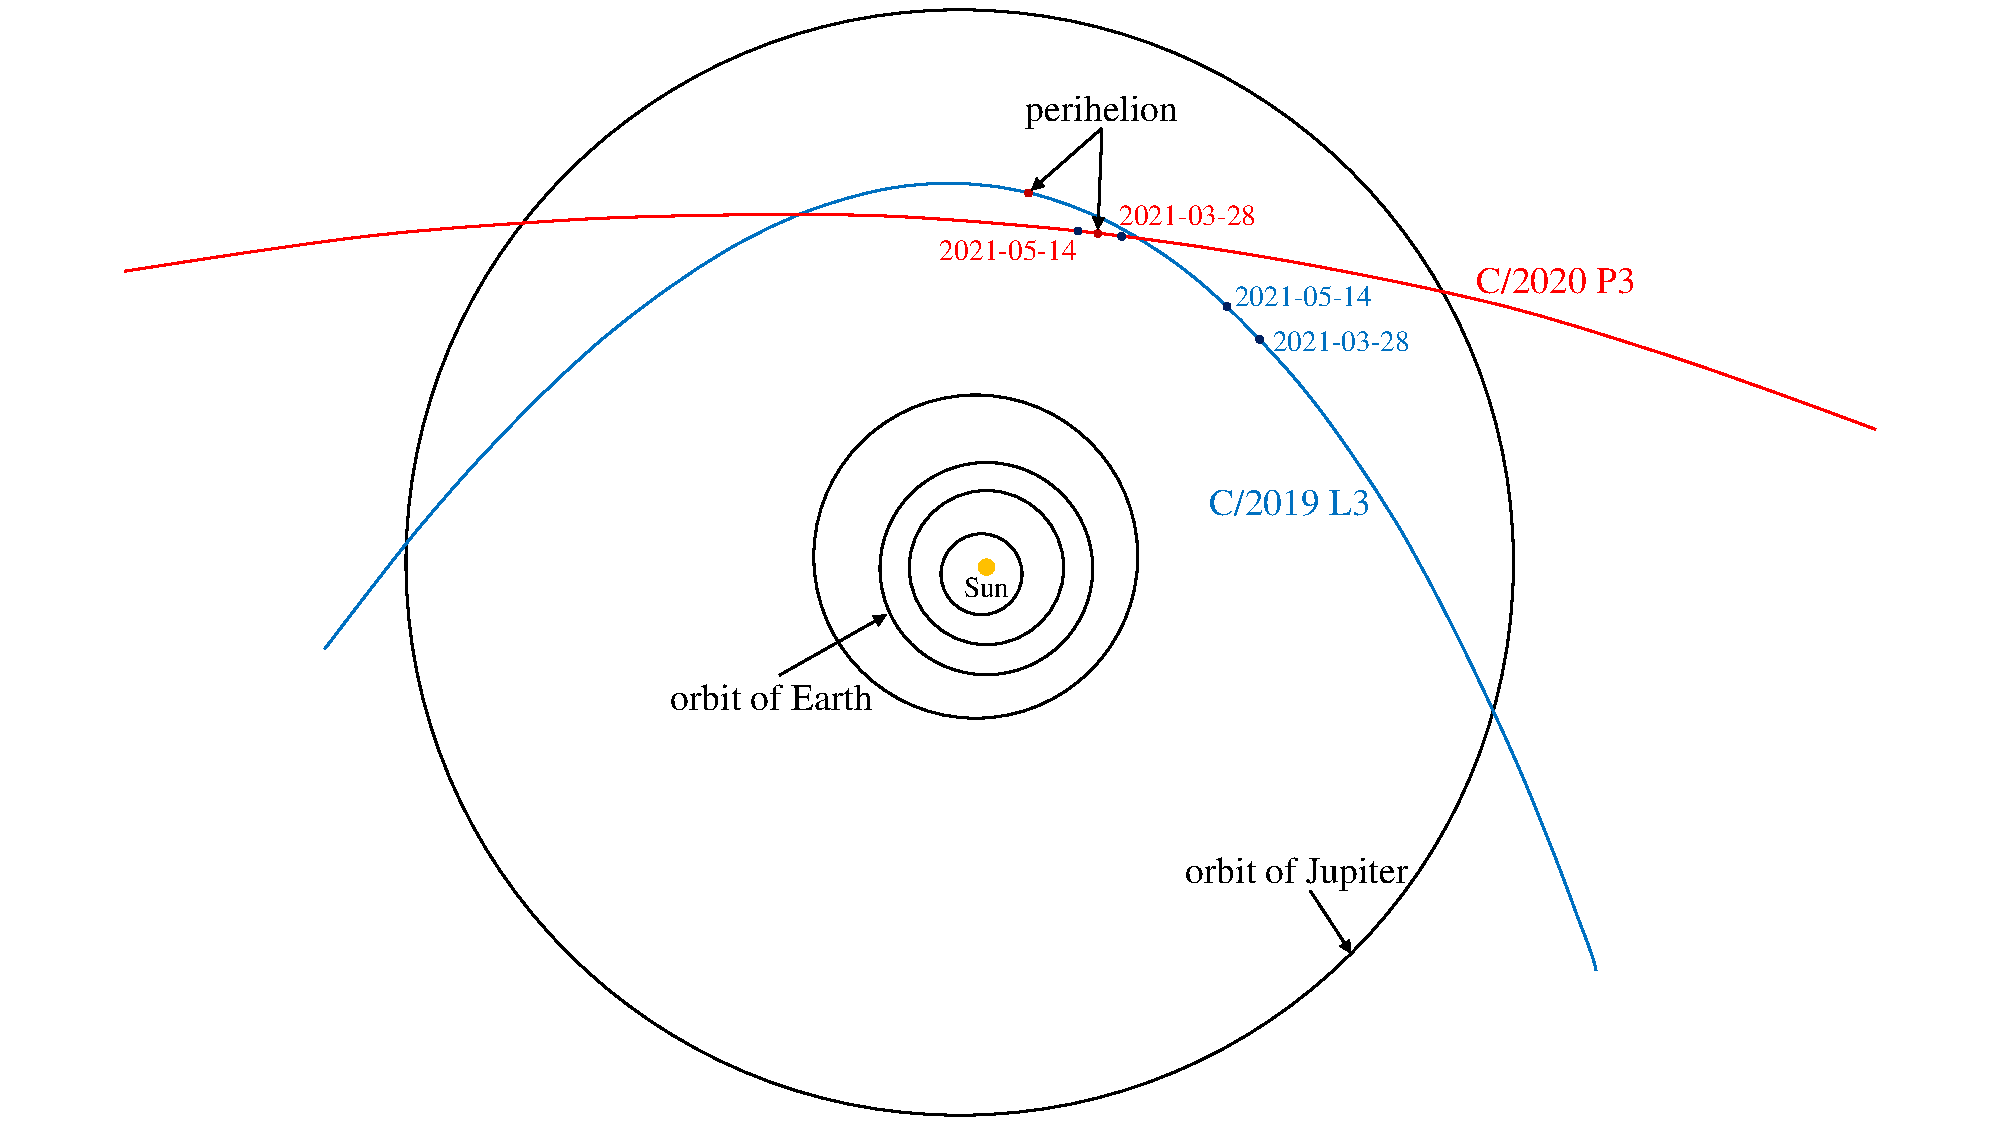
\includegraphics[width=1.0\columnwidth]{orbit.pdf}
    \caption{Orbit of comets C/2019 L3 and C/2020 P3 in the Solar System. The blue curve is the orbit of C/2019 L3 and the red curve is the orbit of C/2020 P3. Closed curves in black are the orbits of planets in the Solar System. Note that both of these comets have large orbital inclination not shown in this planar graph. The start and end dates of observations as well as the corresponding position of two objects on these dates are marked in this graph. }
    \label{fig:orbit}
\end{figure}

% orbital elements
\begin{table}
    \centering
    \caption{Orbital elements of comets C/2019 L3 and C/2020 P3 (Epoch: \DTMdate{2022-7-19}). }\label{tab:orb_elem}
    \begin{threeparttable}
        \resizebox{\linewidth}{!}{
        \begin{tabular}{ccccccccc}
            \toprule
            Comet & e\tnote{1} & q\tnote{2} & i\tnote{3} & $\Omega$\tnote{4} & $\omega$\tnote{5} & L\tnote{6} & B\tnote{7} & T\tnote{8} \\
            \midrule
            C/2019 L3       & \num{1.0017730}  & \num{3.5544290}  & \num{48.35710}  & \num{290.78850}  & \num{171.60970}  & \num{285.19094}  & \num{6.26014}   & \num{2459589.11650}  \\
            C/2020 P3       & \num{1.0003270}  & \num{6.8123330}  & \num{61.88790}  & \num{19.46850}   & \num{82.25590}   & \num{93.37021}   & \num{60.92485}  & \num{2459325.45200} \\
            \bottomrule
        \end{tabular}
        }
% 在正文介绍classification的部分
        \begin{tablenotes}
            \item[1] eccentricity 
            \item[2] perihelion distance
            \item[3] inclination
            \item[4] Longitude of ascending node
            \item[5] Argument of perihelion
            \item[6] Longitude of perihelion
            \item[7] Latitude of perihelion
            \item[8] Time of perihelion passage
        \end{tablenotes}
    \end{threeparttable}
\end{table}


\section{Observations and data reduction} \label{sec:obs_data}

\subsection{Observations}

The observations on two comets metioned above were conducted using three different telescopes belonging to the International Scientific Optical Network (ISON) between 2021 March and 2021 May, namely the {\qty{1.0}{\m}} Zeiss-1000\footnote{\url{https://link.springer.com/content/pdf/10.1134/S1990341320040112.pdf}} 
telescope at Simeiz Observatory (Simeiz), the {\qty{2.6}{\m}} Shajn Telescope (ZTSh\footnote{\url{https://crao.ru/index.php/en/telescopes-en/ztsh-en}}) 
at Crimean Astrophysical Observatory (CrAO), and the {\qty{0.7}{\m}} Maksutov meniscus telescope at Abastumani Astrophysical Observatory (AbAO\footnote{\url{https://www.oato.inaf.it/blazars/webt/abastumani-astrophysical-observatory-georgia-fsu/}}). 
The technical parameters of these telescopes are listed in Table~\ref{tab:telescope}. Four kinds of broadband observational data were obtained with broadband B, V, R and I filters in the Johnson-Cousins system. The log of all observations is presented in Table~\ref{tab:c2019andc2020}. Most of the data were obtained from telescope Maksutov. For comet C/2019 L3, the observations were carried out before the time of perihelion, while for comet C/2020 P3, it was near its perihelion during the observation period. 

% 使用的望远镜信息
\begin{table}
    \centering
    \caption{Information of instrunments used. }\label{tab:telescope}
    \begin{threeparttable}
        \resizebox{\linewidth}{!}{
        \begin{tabular}{ccccccc}
            \toprule
            Telescope & CCD Camera & Focal length [\unit{\mm}] & Frame size & Pixel size & Site & MPC Code\tnote{1} \\
            \midrule
            ZEISS-1000 & FLI & \num{13000} & \makecell[c]{ \qtyproduct{2048 x 2048}{px} \\ $ \ang{;7.3;} \times \ang{;7.3;} $ } & \makecell[c]{\qty{13.5}{\um} \\ \qty{0.216}{^{\prime \prime}/px}}  & Crimea-Simeïs & 094 \\
            ZTSh & FLI PL-4240 & \num{10000} & \makecell[c]{ \qtyproduct{2048 x 2048}{px} \\ $ \ang{;14.2;} \times \ang{;14.2;} $ } & \makecell[c]{ \qty{13.5}{\um} \\ \qty{0.4}{^{\prime \prime}/px}} & Crimea-Nauchnij & 095 \\
            Maksutov & CCD FLI PL4240 & \num{2141} & \qtyproduct{2048 x 2048}{px} & \qty{13.5}{\um} & Abastuman       & 119 \\
            \bottomrule
        \end{tabular}
        }
        \begin{tablenotes}
            \item[1] see Minor Planet Center Observatory Code at \\
            \href{www.minorplanetcenter.net/iau/lists/ObsCodesF.html}{www.minorplanetcenter.net/iau/lists/ObsCodesF.html}
        \end{tablenotes}
    \end{threeparttable}
\end{table}

% 两颗彗星观测数据的总览
\begin{table}
    \centering
    \caption{Log of observations on C/2019 L3 and C/2020 P3}\label{tab:c2019andc2020}
    \begin{threeparttable}
        \resizebox{\linewidth}{!}{
        \begin{tabular}{cccccccc}
            \toprule
            Observation Date & r\tnote{1}~[\si{\astronomicalunit}] & $\Delta$\tnote{2}~[\si{\astronomicalunit}] & Ph.A\tnote{3} & Filters\tnote{4} & Size\tnote{5}~[\si{px}] & Scale\tnote{6}~[\si{\km/px}] & Telescope \\
            \midrule
            \multicolumn{8}{l}{\textbf{C/2019 L3}} \\
            2021-03-28 & 4.385 & 4.916 & 10.4 & B$\times$10, V$\times$10, R$\times$10 & 1018 $\times$ 1018 & 2075 & ZEISS-1000 \\
            2021-04-02 & 4.360 & 4.933 & 10.1 & B$\times$4, V$\times$4, R$\times$5 & 2048 $\times$ 2048 & 4654 & Maksutov \\
            2021-04-03 & 4.355 & 4.936 & 10.1 & B$\times$5, V$\times$5, R$\times$6 & 2048 $\times$ 2048 & 4658 & Maksutov \\
            2021-04-04 & 4.350 & 4.939 & 10.0 & B$\times$10, V$\times$10, R$\times$10 & 2048 $\times$ 2048 & 4660 & Maksutov \\
            2021-04-08 & 4.331 & 4.950 & 9.7 & B$\times$6, V$\times$5, R$\times$5 & 2048 $\times$ 2048 & 4670 & Maksutov \\
            2021-04-12 & 4.311 & 4.960 & 9.5 & B$\times$4, V$\times$5, R$\times$3 & 2048 $\times$ 2048 & 4684 & Maksutov \\
            2021-04-14 & 4.301 & 4.965 & 9.3 & B$\times$4, V$\times$5, R$\times$5 & 2048 $\times$ 2048 & 4686 & Maksutov \\
            2021-04-15 & 4.296 & 4.967 & 9.3 & B$\times$4, V$\times$4, R$\times$4 & 2048 $\times$ 2048 & 4687 & Maksutov \\
            2021-05-04 & 4.205 & 4.987 & 8.0 & B$\times$10, V$\times$10, R$\times$10, I$\times$10 & 1365 $\times$ 1365 & 1587 & ZEISS-1000 \\
            2021-05-10 & 4.177 & 4.985 & 7.6 & B$\times$3, V$\times$3, R$\times$3, I$\times$3 & 2048 $\times$ 2048 & 4709 & Maksutov \\
            2021-05-12 & 4.168 & 4.984 & 7.5 & B$\times$5, V$\times$5, R$\times$5, I$\times$5 & 2048 $\times$ 2048 & 4706 & Maksutov \\
            2021-05-14 & 4.159 & 4.982 & 7.4 & \makecell[c]{B$\times$11, V$\times$11, R$\times$12, I$\times$11 \\ B$\times$7, V$\times$7, R$\times$7, I$\times$7} & \makecell[c]{1024 $\times$ 1024 \\ 2048 $\times$ 2048}  & \makecell[c]{2015 \\ 4706} & \makecell[c]{ZTSh \\ Maksutov} \\

            \multicolumn{8}{l}{\textbf{C/2020 P3}} \\
            2021-03-28\tnote{7} & 6.956 & 6.814 & 8.2 & B$\times$7, V$\times$7, R$\times$7 & 1018 $\times$ 1018 & 2937 & ZEISS-1000 \\
            2021-04-02 & 6.990 & 6.813 & 8.2 & V$\times$11, R$\times$14 & 2048 $\times$ 2048 & 6592 & Maksutov \\
            2021-05-11 & 7.216 & 6.814 & 7.6 & C$\times$4, V$\times$5, R$\times$5 & 2048 $\times$ 2048 & 6807 & Maksutov \\
            2021-05-12 & 7.221 & 6.814 & 7.6 & \makecell[c]{B$\times$3, V$\times$3, R$\times$3, I$\times$3 \\ B$\times$6, V$\times$5, R$\times$5, I$\times$5} & \makecell[c]{1024 $\times$ 1024 \\ 2048 $\times$ 2048}  & \makecell[c]{2914 \\ 6807} & \makecell[c]{ZTSh \\ Maksutov} \\
            \bottomrule
        \end{tabular}
        }
        \begin{tablenotes}
            \item[1] heliocentric distance
            \item[2] geocentric distance
            \item[3] phase angle
            \item[4] numbers after `$\times$' indicate amounts of images under corresponding filters, \\
            `C' means `clear glass'
            \item[5] size of original image
            \item[6] the calculated image scale in \si{\km} per pixel
            \item[7] images on this date are too faint to use
        \end{tablenotes}
    \end{threeparttable}
\end{table}

\subsection{Data reduction}

All of the images had been corrected with common methods for dark subtraction, bias subtraction and flat-field normalization when ISON provided the observational data for this research. In order to \st{raise} \ul{improve} the signal-to-noise ratio, images on different observational dates were aligned and sum combined for different filters according to the photocenter of comet. The same thing was also done on the basis of photocenter of background star as the motion of comet in each frame is obvious. Several tasks such as \texttt{center}, \texttt{imshift} and \texttt{combine} in IRAF (the \textbf{I}mage \textbf{R}eduction and \textbf{A}nalysis \textbf{F}acility)\footnote{\url{https://github.com/iraf-community/iraf}}, were applied for this procedure. Since the comet and reference stars for photometry are in the same frame, the airmass correction \st{is not necessary} \ul{can be neglected}. Given that some images are in the case where comet gets too close to the background stars around, psf subtraction was conducted to cover up these stars with tasks such as \verb|substar|. 

The photometric calibration of these two comets' data was performed with the UCAC4 \citep{zacharias_fourth_2013} and UCAC5 \citep{zacharias_ucac5_2017}. Additionally, the GCVS 5.1 \citep{samus_general_2017} was applied to inspect the variability of all the comparison stars. 

In order to measure the  instrunment magnitudes of comets and comparison stars, circular aperture photometry was applied. When conducting aperture photometry on stars, the sky background value is determined by the annular region around the star. However, when conducting aperture photometry on comets, the sky background value is determined by several clean background areas far away from the comet. The photometric aperture of comparison stars was determined by nearly \si{\num{2}} times the full-wide at half-maximum (FWHM). Since three different telescopes were involved during the observation, the photometry of comets was performed on different apertures centered on the comet photocenter, with all of them ensured to be up to \si{\num{1.5}} times the full-wide at half-maximum and close to each other in arcsecond as much as possible. 
The ranges of seeings for the three telescopes are as follows: \ang{;;1.2} to \ang{;;7.5} for ZEISS-1000, \ang{;;3.9} to \ang{;;11.7} for Maksutov, and \ang{;;2.4} to \ang{;;3.9} for ZTSh. 
The photometric results are listed as Table~\ref{tab:bvr}, and the error of photometry $e_{\mathrm{phot}}$ is derived from equation (\ref{eq:err}) as follows: 
\begin{equation}
    e_{\mathrm{phot}} = \sqrt{e_{\mathrm{c}}^{2} + \sigma_\mathrm{s}^2}, 
    \label{eq:err}
\end{equation}
where $e_\mathrm{c}$ is the magnitude error of comet from IRAF photometric file and $\sigma_\mathrm{s}$ is the standard deviation of the calibration values in differential photometry. 








\section{Results} \label{sec:res}

\subsection{Morphology}

The original images of C/2019 L3 in the R band exhibit greater clarity compared to images in other bands, and they all resemble a star-like appearance. On the other hand, the original images of C/2020 P3 appear very faint, and the ones taken in the R band are also relatively clearer than those in other bands. Unlike C/2019 L3, some images of C/2020 P3 reveal the presence of an extended tail. After applying the data reduction process mentioned before, we get one image for each filter on each observational date. Fig.~\ref{fig:combinedimg} is a thumbnail view of the reduction result with comet located in center of each small parts whose field of view are all $\ang{;2;} \times \ang{;2;}$. On \DTMdate{2021-5-14}, images of comet C/2019 L3 were taken by two telescope, thus in Fig.~\ref{fig:combinedimg} there are two groups of thunbnails on this date with the upper one by telescope ZTSh and the lower one by telescope Maksutov, so were images of comet C/2020 P3 on \DTMdate{2021-5-12}. The black spots in several part of this view are due to the psf subtraction process, as it is not always perfect for star subtraction. For comet C/2019 L3, the observational record is abundant. The I band filter was added in the observation from May, 2021, providing more data for this study. From the combined images of C/2019 L3, it is easily to notice that this comet is very round and seemingly isotropic. For comet C/2020 P3, there are few data and in some cases it is hard to identify in single image. However, its extended coma looking like a tail is more obvious, especially for the images taken on \DTMdate{2021-5-12}, which roughly measured \ang{;;20} from comet center in R-band image. 

For morphology analysis, it is necessasy to apply some image enhancement techniques with which we can recognize some features and structures hidden in \st{background} \ul{coma} \citep{samarasinha_image_2014}. Many pieces of software have been developed for comet image enhancement, such as {\href{https://www.msb-astroart.com/down_en.htm}{Astroart 8}} and online tool {\href{https://www.psi.edu/research/cometimen}{Cometary Coma Image Enhancement Facility}}. In this work, 
we applied azimuthal renormalization method on images of C/2019 L3 on \DTMdate{2021-5-14} by telescope Maksutov since other images are too faint and show no evident features after enhanced. The result is shown in Fig.~\ref{fig:aziren}, where the enhanced images under V and R filters show a small northeastward fan-shape structure, while the enhanced images under B and I filters give no obvious feature.  

\begin{figure}
    \centering
    \subcaptionbox{C/2019 L3: BVR}[\linewidth]{
        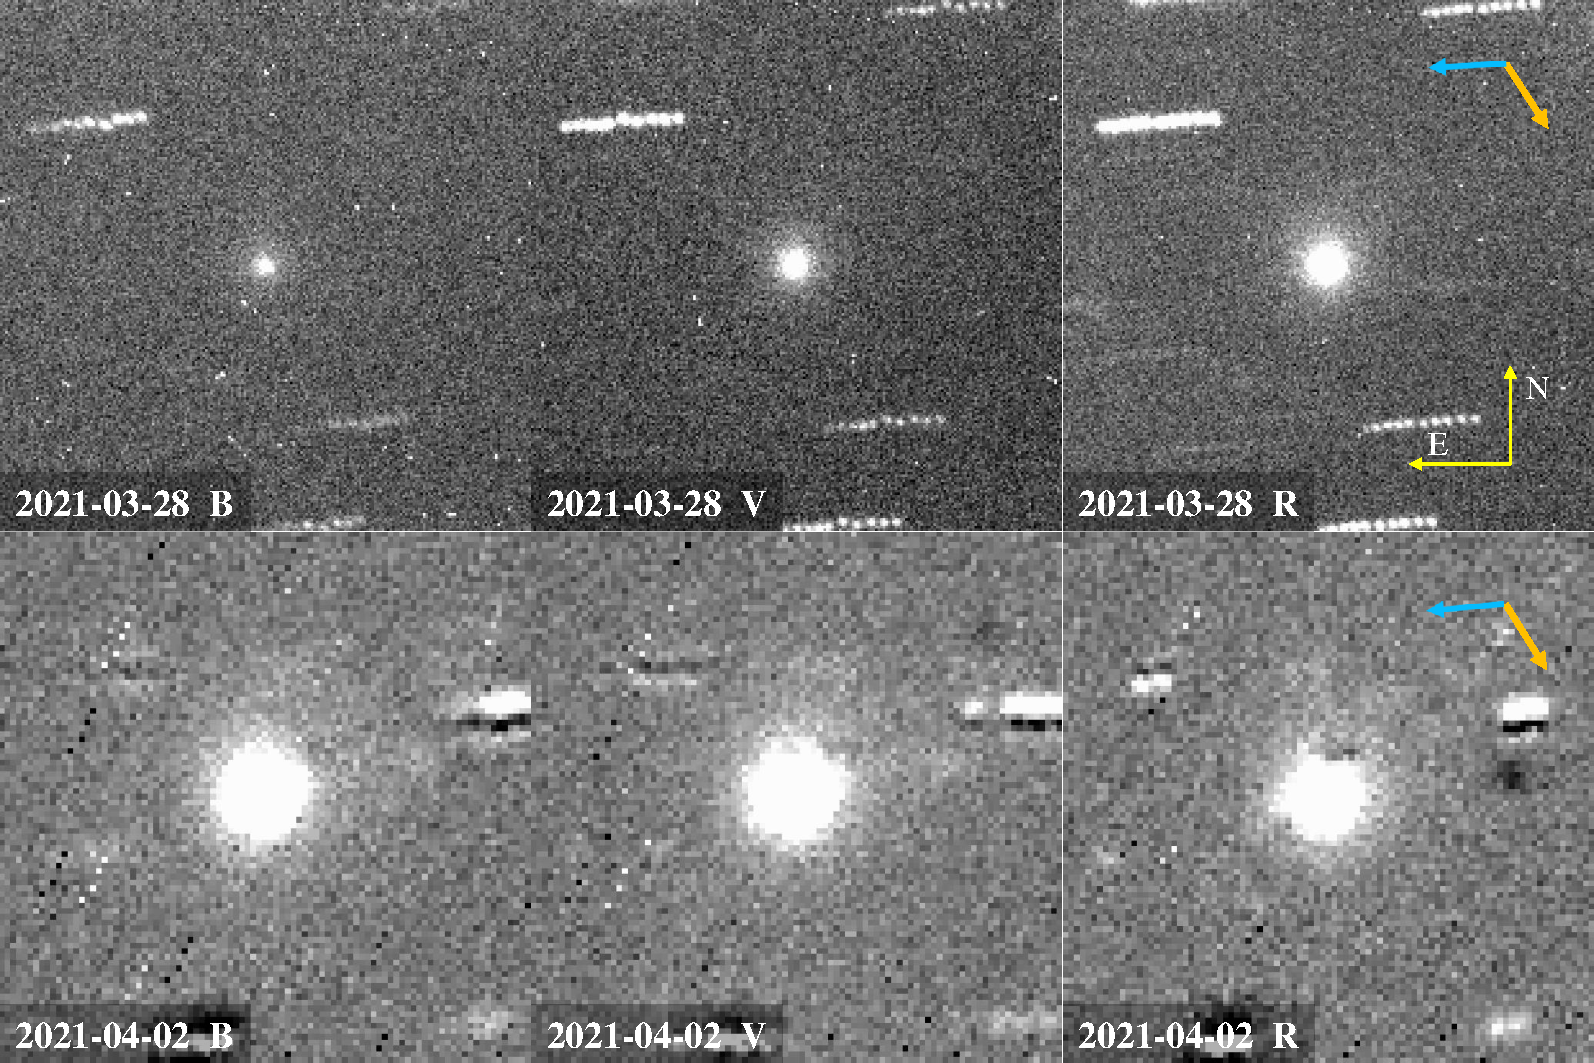
\includegraphics[width=.9\linewidth]{combine1.pdf}
        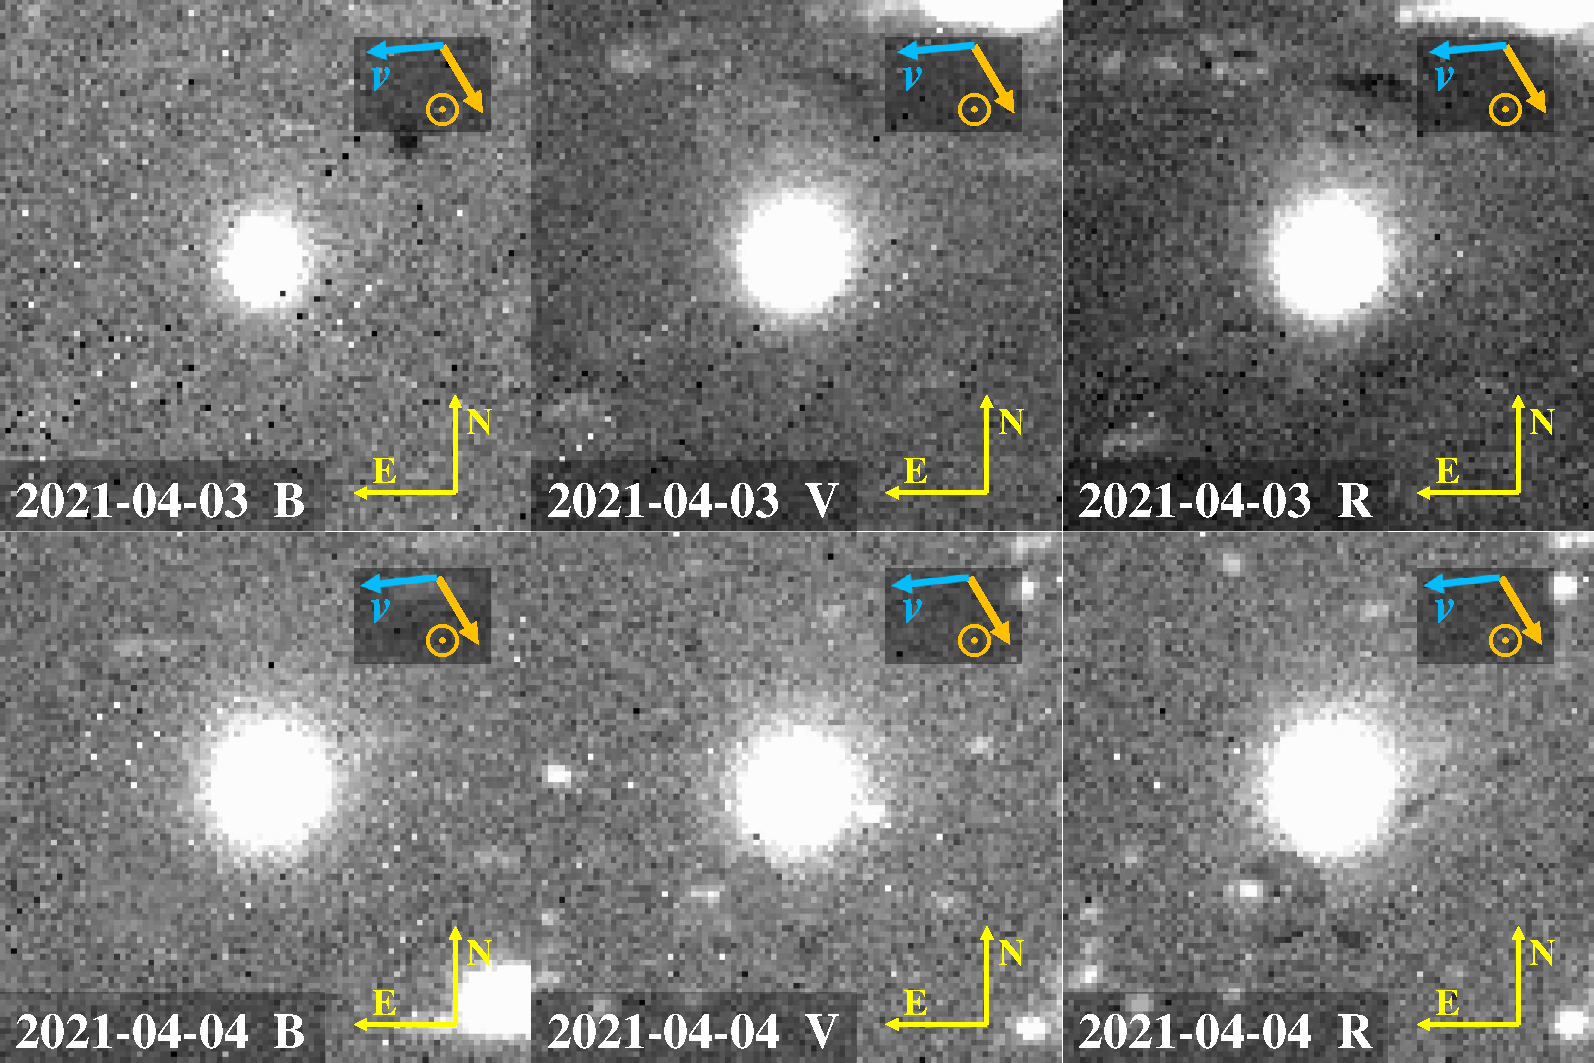
\includegraphics[width=.9\linewidth]{combine2.pdf} 
        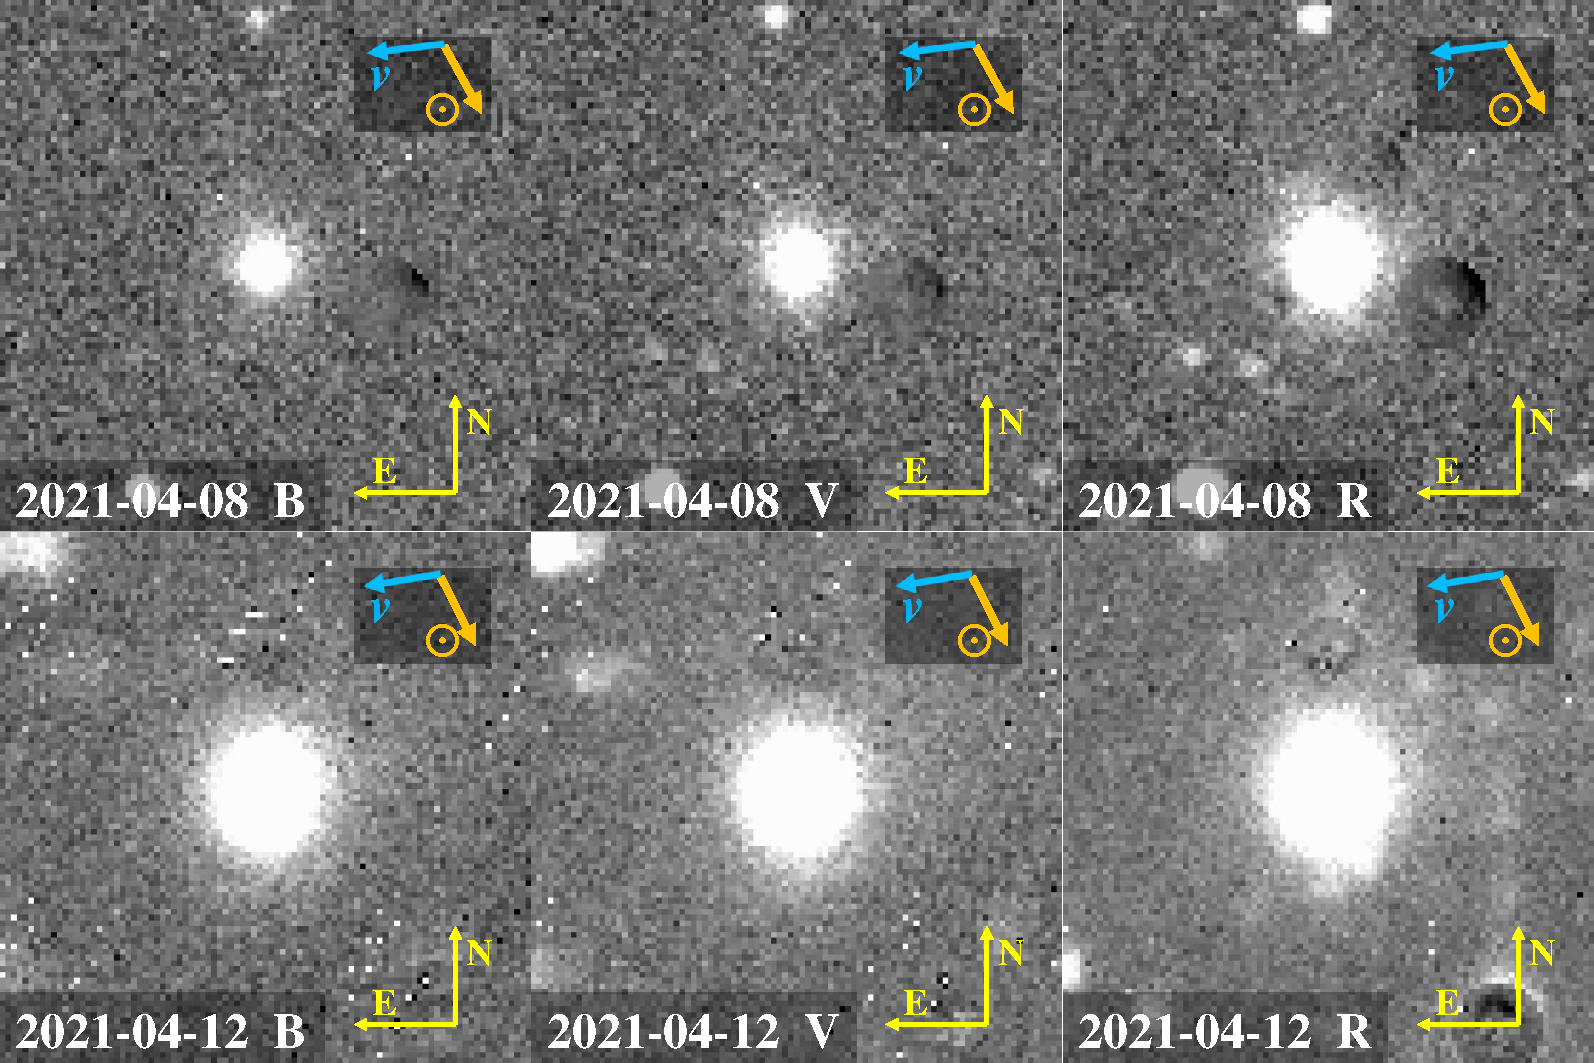
\includegraphics[width=.9\linewidth]{combine3.pdf}
        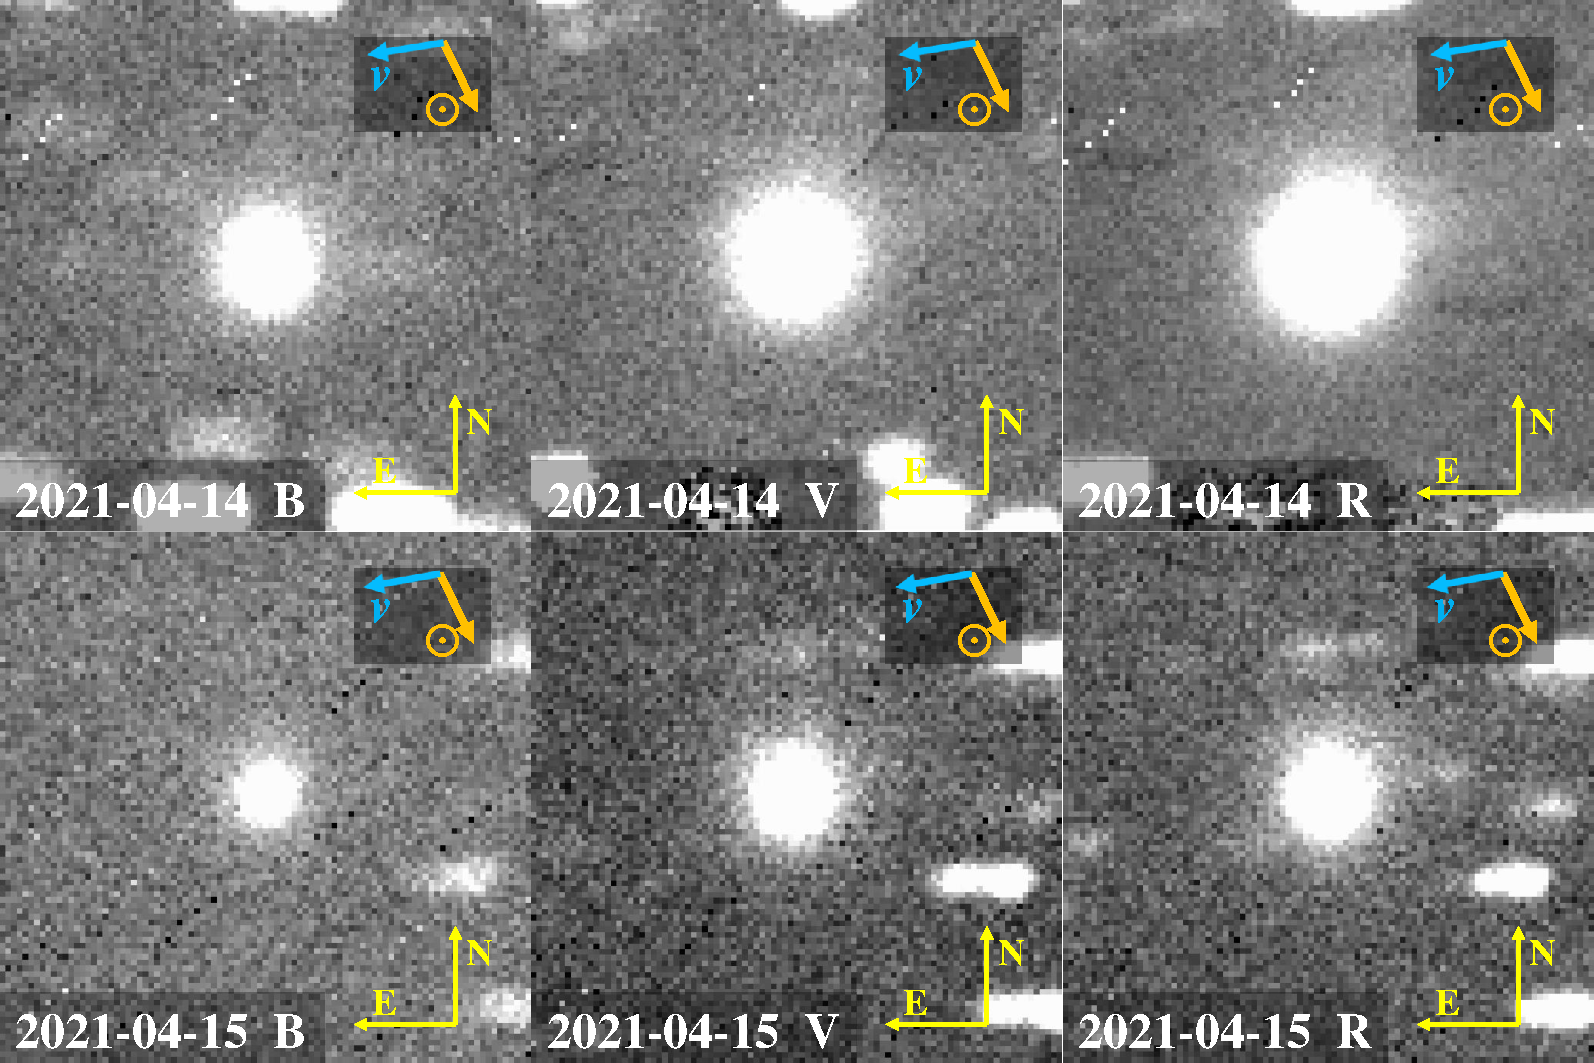
\includegraphics[width=.9\linewidth]{combine4.pdf}
    }
    \caption{The processed images of comet C/2019 L3 and C/2020 P3 in different filters, with north at the top and east to the left. The field of view is $ 2^{\prime} \times 2^{\prime} $ for each thumbnail. Blue arrow shows the direction of the comets' velocity, and the orange arrow shows the direction to the Sun. }
    \label{fig:combinedimg}
\end{figure}

\begin{figure}
    \centering
    \ContinuedFloat
    \subcaptionbox{C/2019 L3: BVRI}[\linewidth]{
        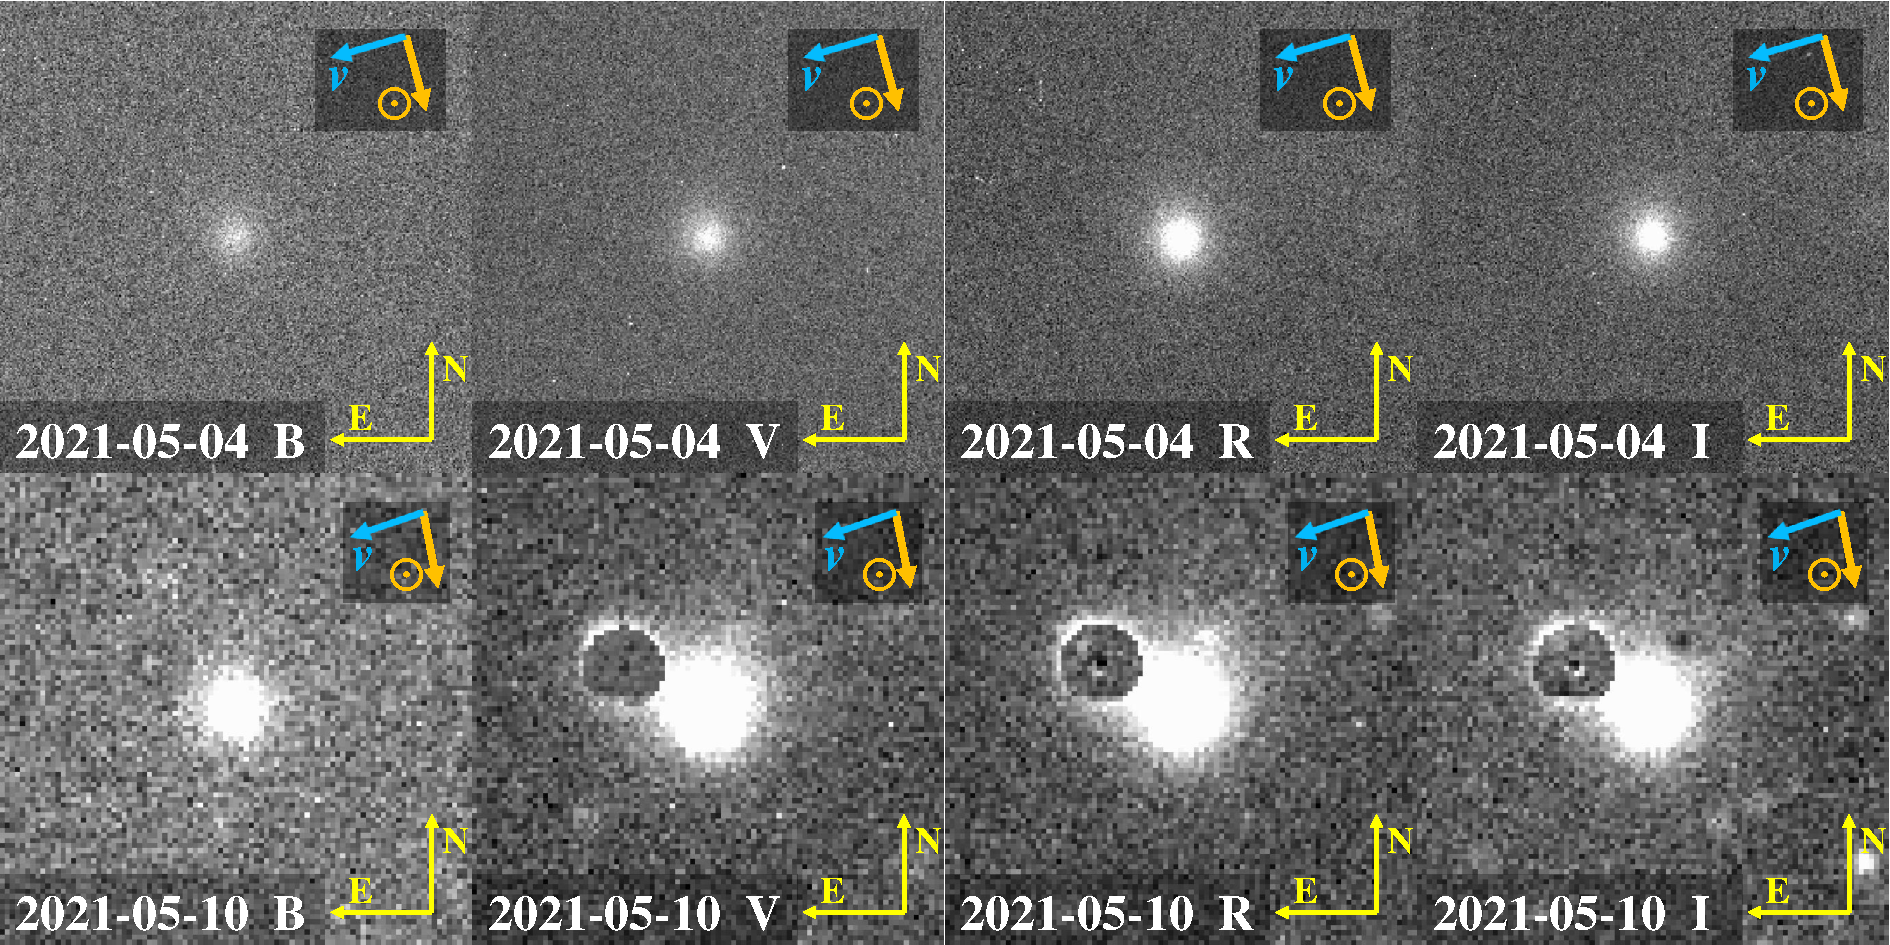
\includegraphics[width=\linewidth]{combine5.pdf}
        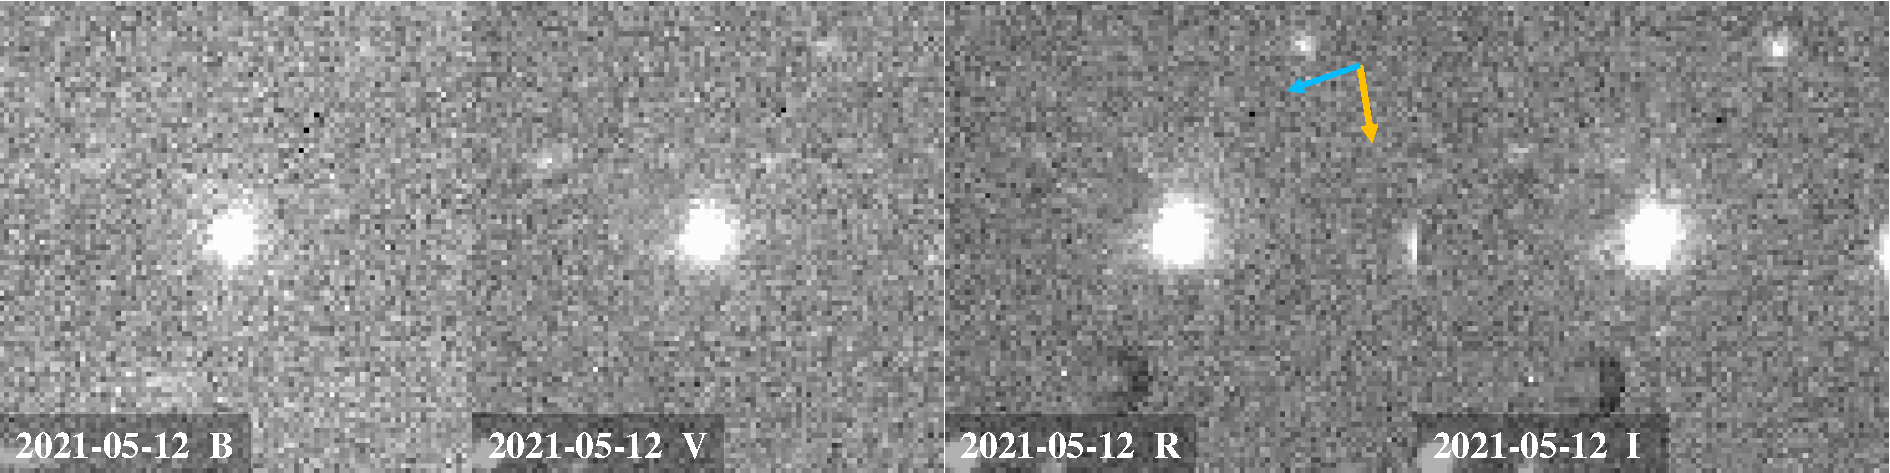
\includegraphics[width=\linewidth]{combine6.pdf} 
        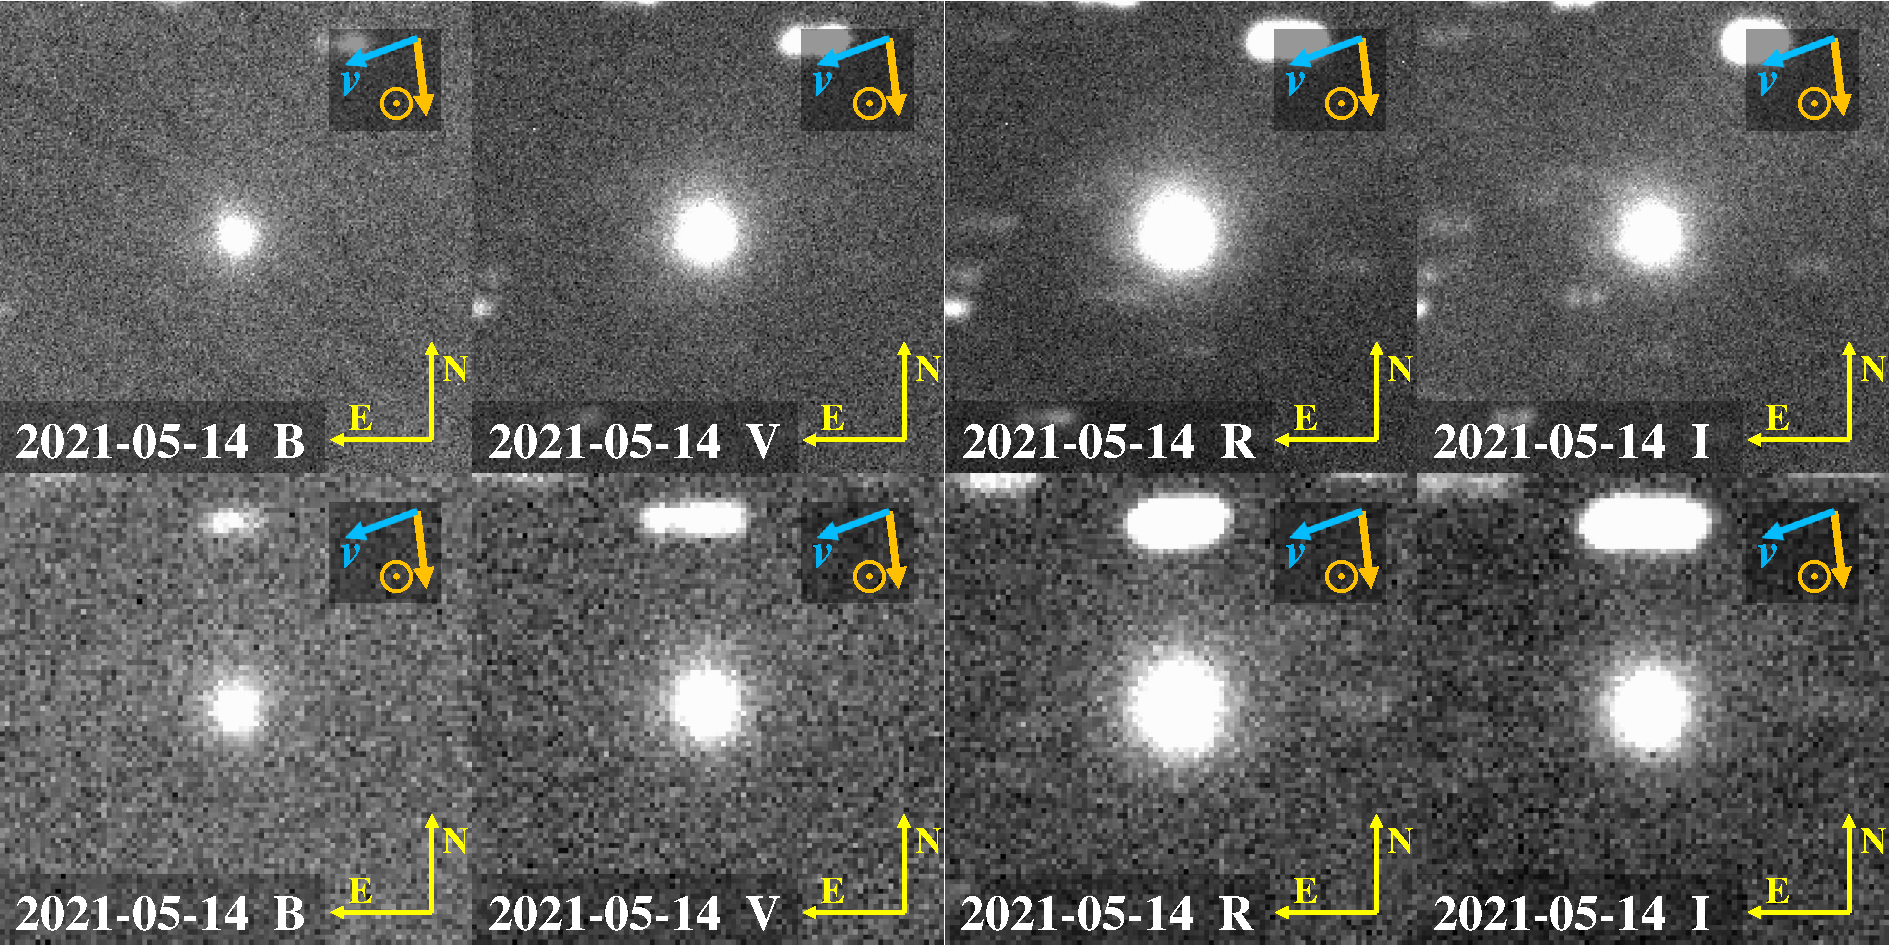
\includegraphics[width=\linewidth]{combine7.pdf} 
    }
        
    \caption{(Continued)}
\end{figure}

\begin{figure}
    \centering
    \ContinuedFloat
    \subcaptionbox{C/2020 P3}[\linewidth]{
        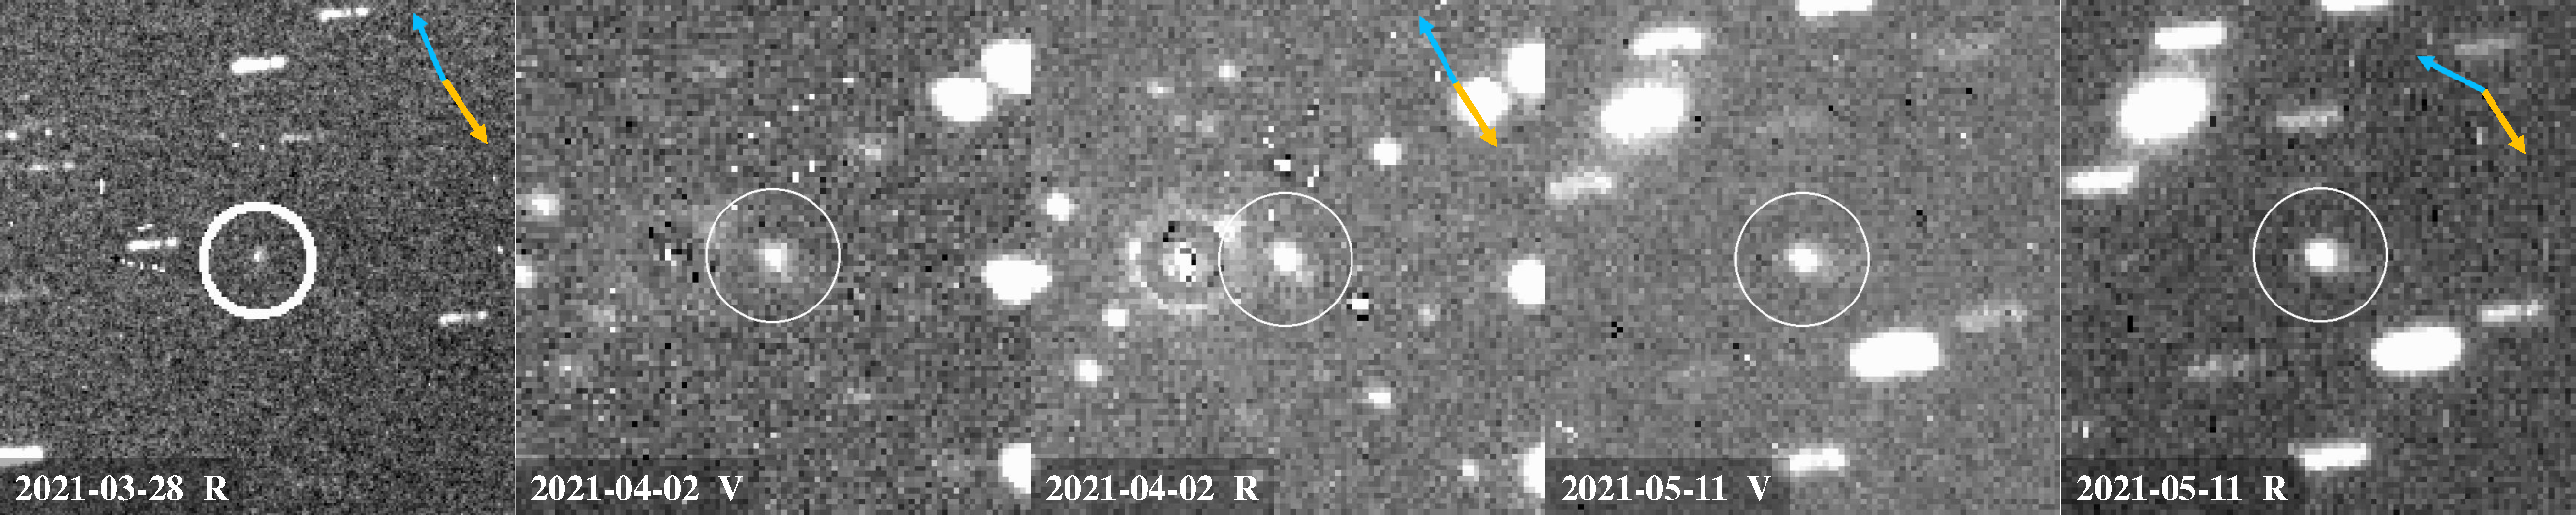
\includegraphics[width=\linewidth]{combine8.pdf}
        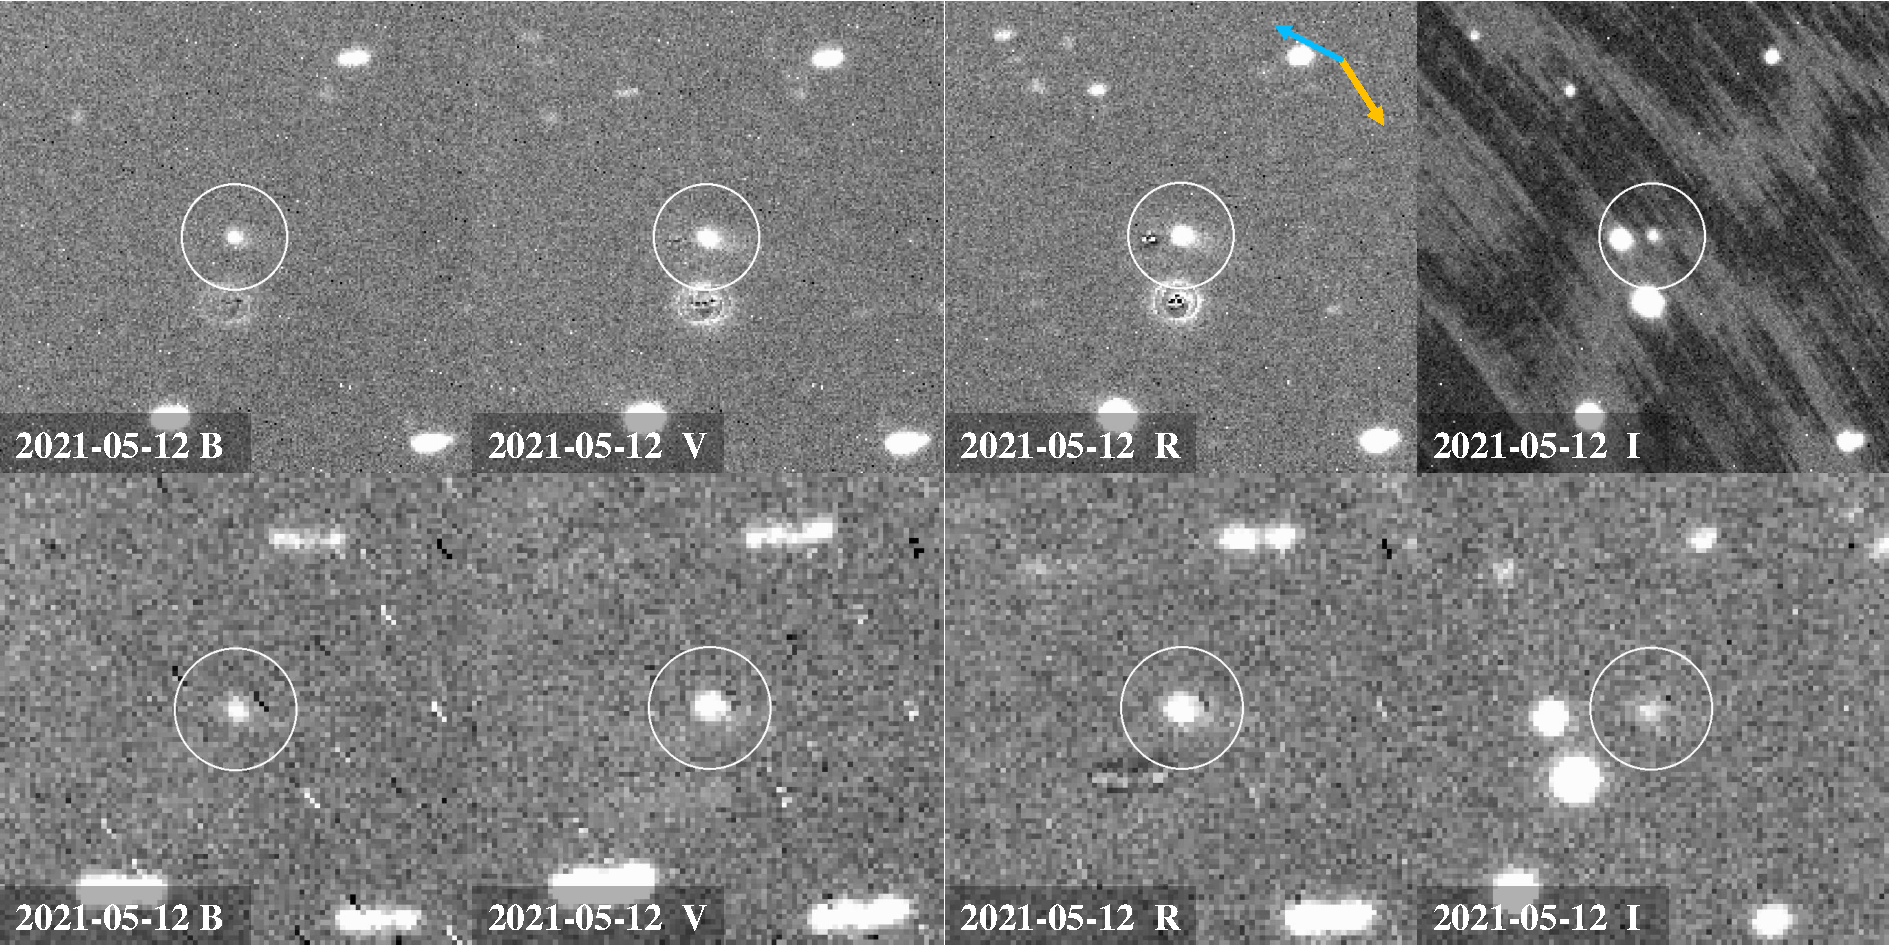
\includegraphics[width=\linewidth]{combine9.pdf} 
    }
    
    \caption{(Continued)}
\end{figure}

\begin{figure}
    \centering
    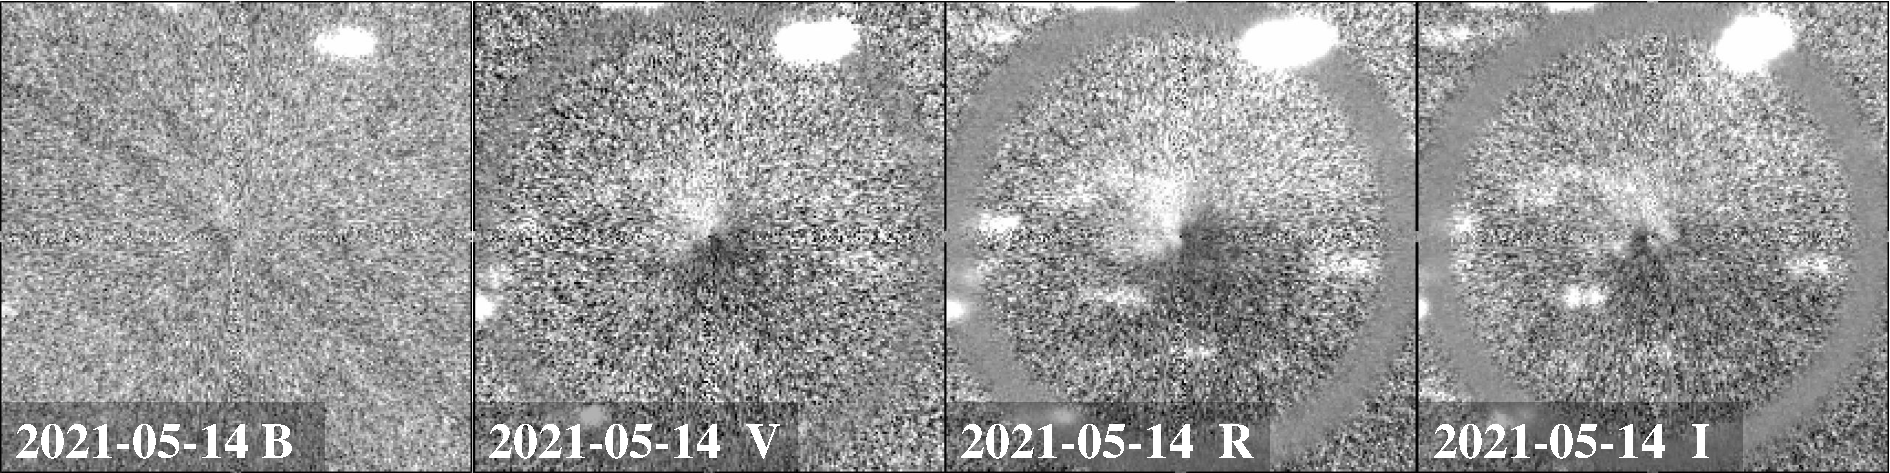
\includegraphics[width=\linewidth]{azi_ren.pdf}
    \caption{Azimuthal renormalized image of C/2019 L3 on \DTMdate{2021-5-14}, the field of view for each thunbnail is also $\ang{;2;}\times\ang{;2;}$. \label{fig:aziren}}
\end{figure}
    
% BVR
\begin{table}
    \centering
    \caption{Photometric results of comet C/2019 L3 and C/2020 P3. }\label{tab:bvr}
    \begin{threeparttable}
        \resizebox{\linewidth}{!}{
        \begin{tabular}{ccccccccc}
            \toprule
            Observation Time\tnote{1} & $\rho\tnote{2}~[^{\prime \prime}]$ & B & V & R & I & $\mathrm{B}-\mathrm{V}$ & $\mathrm{V}-\mathrm{R}$ & $\mathrm{R}-\mathrm{I}$\\
            \midrule
            \multicolumn{9}{l}{\textbf{C/2019 L3}} \\
            2021-03-28.729 & 14.5 & \num{14.32 +- 0.09} & \num{13.72 +- 0.07} & \num{13.17 +- 0.15} & - & \num{0.60 +- 0.11} & \num{0.55 +- 0.16} & - \\
            2021-04-02.739 & 15.6 & \num{14.37 +- 0.10} & \num{13.62 +- 0.04} & \num{13.14 +- 0.06} & - & \num{0.75 +- 0.11} & \num{0.48 +- 0.07} & - \\
            2021-04-03.719 & 15.6 & \num{14.25 +- 0.05} & \num{13.55 +- 0.03} & \num{13.08 +- 0.07} & - & \num{0.70 +- 0.05} & \num{0.47 +- 0.08} & - \\
            2021-04-04.691 & 15.6 & \num{14.26 +- 0.05} & \num{13.55 +- 0.02} & \num{13.32 +- 0.01} & - & \num{0.70 +- 0.05} & \num{0.23 +- 0.02} & - \\
            2021-04-08.691 & 15.6 & \num{14.33 +- 0.05} & \num{13.44 +- 0.02} & \num{13.36 +- 0.01} & - & \num{0.88 +- 0.05} & \num{0.09 +- 0.03} & - \\
            2021-04-12.724 & 19.5 & \num{14.22 +- 0.05} & \num{13.33 +- 0.01} & \num{13.19 +- 0.01} & - & \num{0.89 +- 0.05} & \num{0.14 +- 0.02} & - \\
            2021-04-14.702 & 15.6 & \num{14.21 +- 0.04} & \num{13.51 +- 0.03} & \num{13.29 +- 0.02} & - & \num{0.71 +- 0.05} & \num{0.21 +- 0.03} & - \\
            2021-04-15.714 & 15.6 & \num{14.23 +- 0.03} & \num{13.51 +- 0.01} & \num{13.28 +- 0.02} & - & \num{0.72 +- 0.04} & \num{0.23 +- 0.02} & - \\
            2021-05-04.736 & 11.0 & \num{14.32 +- 0.04} & \num{13.75 +- 0.04} & \num{13.42 +- 0.04} & \num{13.25 +- 0.03} & \num{0.57 +- 0.05} & \num{0.33 +- 0.06} & \num{0.17 +- 0.05} \\
            2021-05-10.735 & 15.6 & \num{13.96 +- 0.03} & \num{13.24 +- 0.01} & \num{13.05 +- 0.03} & \num{12.80 +- 0.04} & \num{0.72 +- 0.04} & \num{0.18 +- 0.03} & \num{0.26 +- 0.05} \\
            2021-05-12.724 & 15.6 & \num{14.14 +- 0.03} & \num{13.27 +- 0.03} & \num{13.11 +- 0.02} & \num{12.90 +- 0.03} & \num{0.87 +- 0.05} & \num{0.16 +- 0.04} & \num{0.22 +- 0.04} \\
            2021-05-14.721 & 14.0 & \num{14.21 +- 0.04} & \num{13.28 +- 0.04} & \num{13.13 +- 0.02} & \num{12.90 +- 0.06} & \num{0.93 +- 0.06} & \num{0.15 +- 0.04} & \num{0.24 +- 0.06} \\
            \multicolumn{9}{l}{\textbf{C/2020 P3}} \\
            2021-04-02.775 & 13.0 & - & \num{17.61 +- 0.05} & \num{17.24 +- 0.03} & - & - & \num{0.37 +- 0.05} & - \\
            2021-05-11.744 & 13.0 & - & \num{18.15 +- 0.05} & \num{17.83 +- 0.04} & - & - & \num{0.32 +- 0.06} & - \\
            2021-05-12.749 & 6.7 & \num{19.00 +- 0.06} & \num{18.05 +- 0.03} & \num{17.88 +- 0.02} & \num{17.67 +- 0.04} & \num{0.95 +- 0.07} & \num{0.17 +- 0.04} & \num{0.21 +- 0.05} \\
            \bottomrule
        \end{tabular}
        }
        \begin{tablenotes}
            \item[1] UT time at the beginning of exposure
            \item[2] the photometric aperture in arcsecond
        \end{tablenotes}
    \end{threeparttable}
\end{table}

\begin{comment}
\subsection{Nucleus size}

For comets observed at large heliocentric distances that are commonly assumed to be inactive, their photometric R magnitude, denoted as $m_R$, can be utilized to derive the maximum estimate for the geometric cross-sectional area of the cometary nucleus. This estimation involves the use of the formula proposed by \cite{lamy_comet_2004} for asteroids observed at high phase angle that can be applied to a spherical body expressed as
\begin{equation}
    A_R a_N^2 < \num{2.24e22} r^2 \Delta^2 10^{0.4\left(m_{\odot} - m_R + \beta \alpha\right)}, 
\end{equation}
where $A_R = 0.04$ is the geometric albedo \citep{lamy_comet_2004}, $a_N$ the radius, $r$ the heliocentric distance in \si{\astronomicalunit}, $\Delta$ the geocentric distance in \si{\astronomicalunit}, $m_{\odot} = -27.15$ the R magnitude of the Sun \citep{willmer_absolute_2018}, $\alpha$ the phase angle, and $\beta = 0.04$ the phase coefficient \citep{lamy_comet_2004}. 
Given that two comets in this work were active during the observational run, we set the photometry aperture equal to stellar FWHM and calculate the background value using a circular region near the comet nucleus to reduce the influence of cometary outbursts, then use differential photometry to get new R magnitude to provide a coarse estimation for the nucleus size. 
The images of comet C/2019 L3 taken on \DTMdate{2021-5-4} and that of C/2020 P3 taken on \DTMdate{2021-5-12} exhibit high resolution and were captured at sufficiently distant heliocentric distance, from which we were able to estimate the upper limits of radii for two comets as follows: C/2019 L3 with a limit of {\SI{75.1 +- 3.5}{\km}}, and C/2020 P3 with a limit of {\SI{26.8 +- 0.7}{\km}}. 

% 在后面讨论一下减除彗发的方法是否可靠 (是否稳态彗发? 稳态时可靠)
\end{comment}

\subsection{Surface brightness profile}

Based on the photometric results, the radial surface brightness profile (SBP) was computed as the function of the angular distance $\rho$ measured from the photocenter of comet. For this purpose, every image was trimmed from the center of the comet, and the sky value was determined by the median of the trimmed image. 
In the case of a steady-state coma, the surface brightness $B$ is expected to follow a power-law relation with $\rho$ as $B \propto \rho^m$, where $-1.5 \leqslant m \leqslant -1.0$, and the index $m$ is often referred to as the gradient ($m=\dif\lg{B} / \dif\lg{\rho}$). As the radiation pressure accelerates the dust particles, the value of $m$ decreases and approaches \si{\num{-1.5}} in the limiting case~\citep{jewitt_surface_1987}. Conversely, if the index $m$ falls below \si{\num{-1.5}}, it suggests the presence of nonsteady dust coma emission.

Not only in single images does comet C/2019 L3 appear like a stellar, but also in stacked images. However, the SBP of C/2019 L3 shows it clearly the excess flux in outer region compared with stellar SBP. In Fig.~\ref{fig:sbp} we report an example plot of the R-band SBP as a function of $\lg{\rho}$ for C/2019 L3 observed on \DTMdate{2021-5-4}. The gradient $m$ in the $0.5 \leqslant \lg{\rho} \leqslant 1.0$ range is calculated by the least-squares fit to $\lg{B}$ versus $\lg{\rho}$. 
In Fig.~\ref{fig:sbp_m}, the gradients of C/2019 L3 on each date are depicted, and the averaged value is indicated by a blue dotted line. 
Note that in Fig.~\ref{fig:sbp} the SBP is expressed as magnitude, and according to the relationship between magnitude and luminous intensity, the slope in such figure should be multiplied by \num{-0.4} to make the gradient $m$. The averaged $m$ is \si{\num{-1.68}}, and in most cases it is below \si{\num{-1.5}}, indicating that this comet's dust emission is in a nonsteady state. While for comet C/2020 P3, all images taken are so faint and it would bring about a great deal of uncertainty if we calculated its SBP. 

% 考虑放置最大、最小、中位数对应图像
\begin{figure}
    \centering
    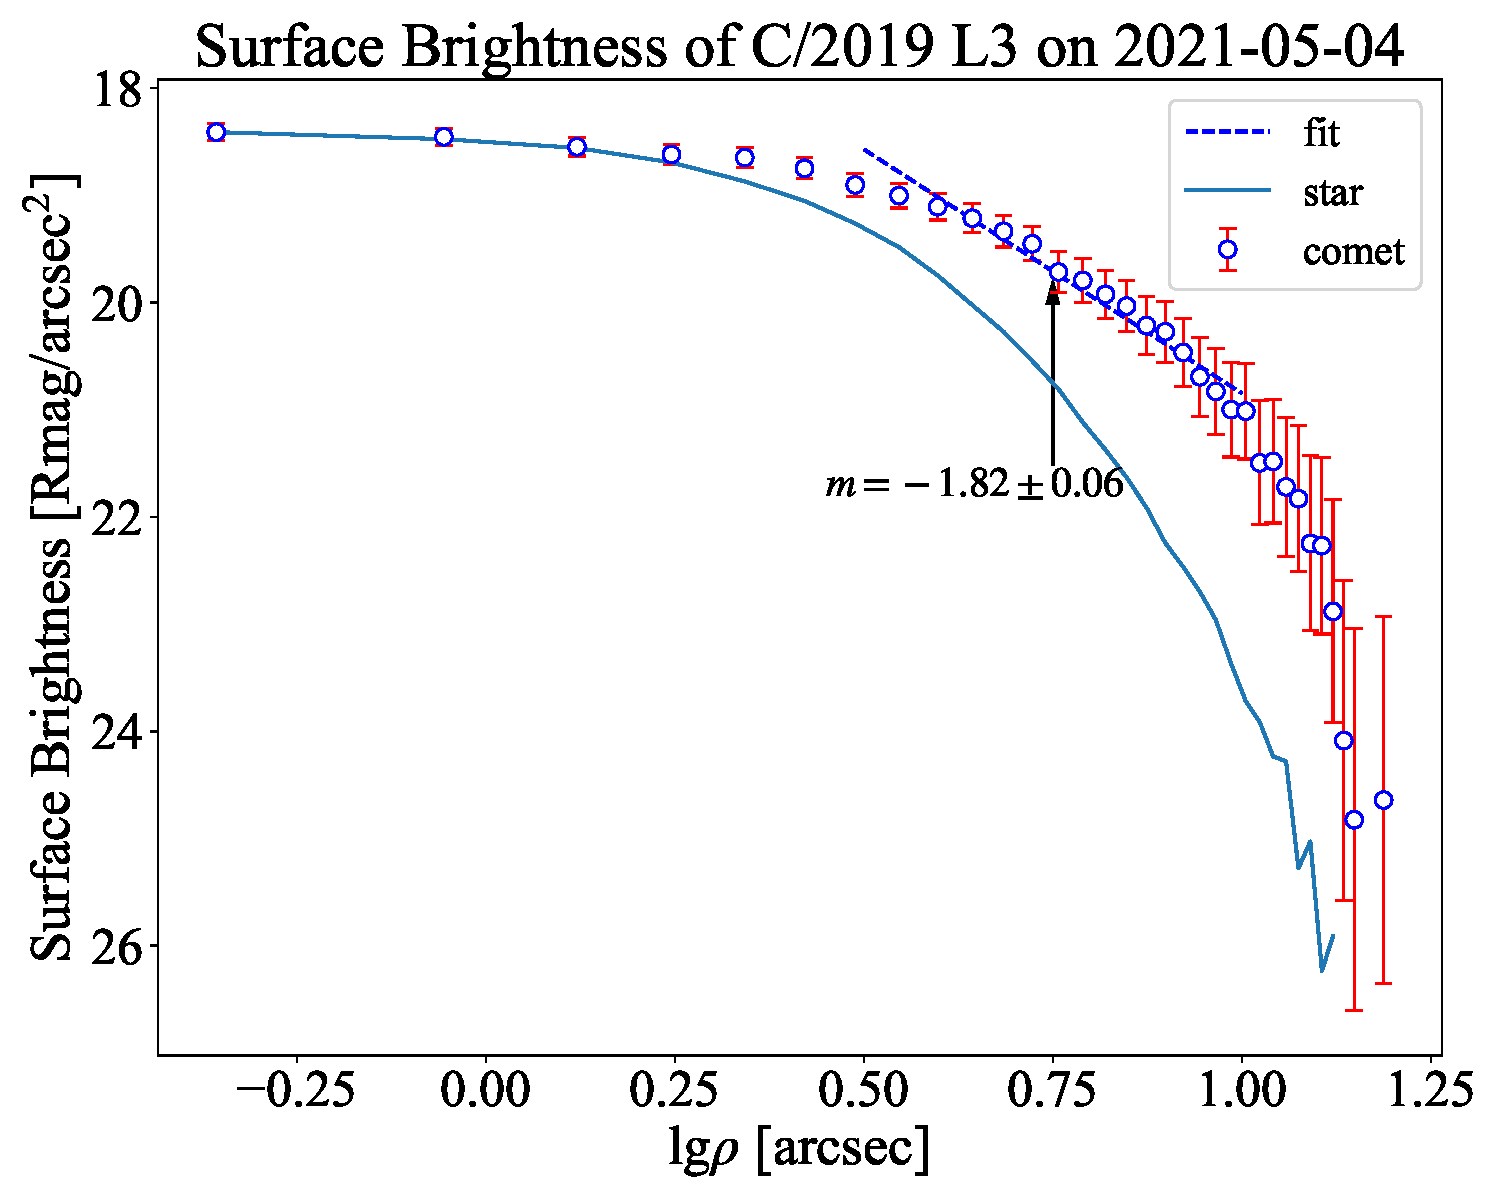
\includegraphics[width=\columnwidth]{sbp-210504.pdf}
    \caption{An example figure for R-band surface brightness of comet C/2019 L3. The error plot is the SBP of comet, and the blue solid line is the SBP of a background star. The blue dotted line is a linear regression result of comet's SBP vs $\lg{\rho}$ with $\lg{\rho}$ between 0.5 and 1.0, and the gradient $m$ related to the slope is marked on the graph with an arrow. }
    \label{fig:sbp}
\end{figure}

\begin{figure}
    \centering
    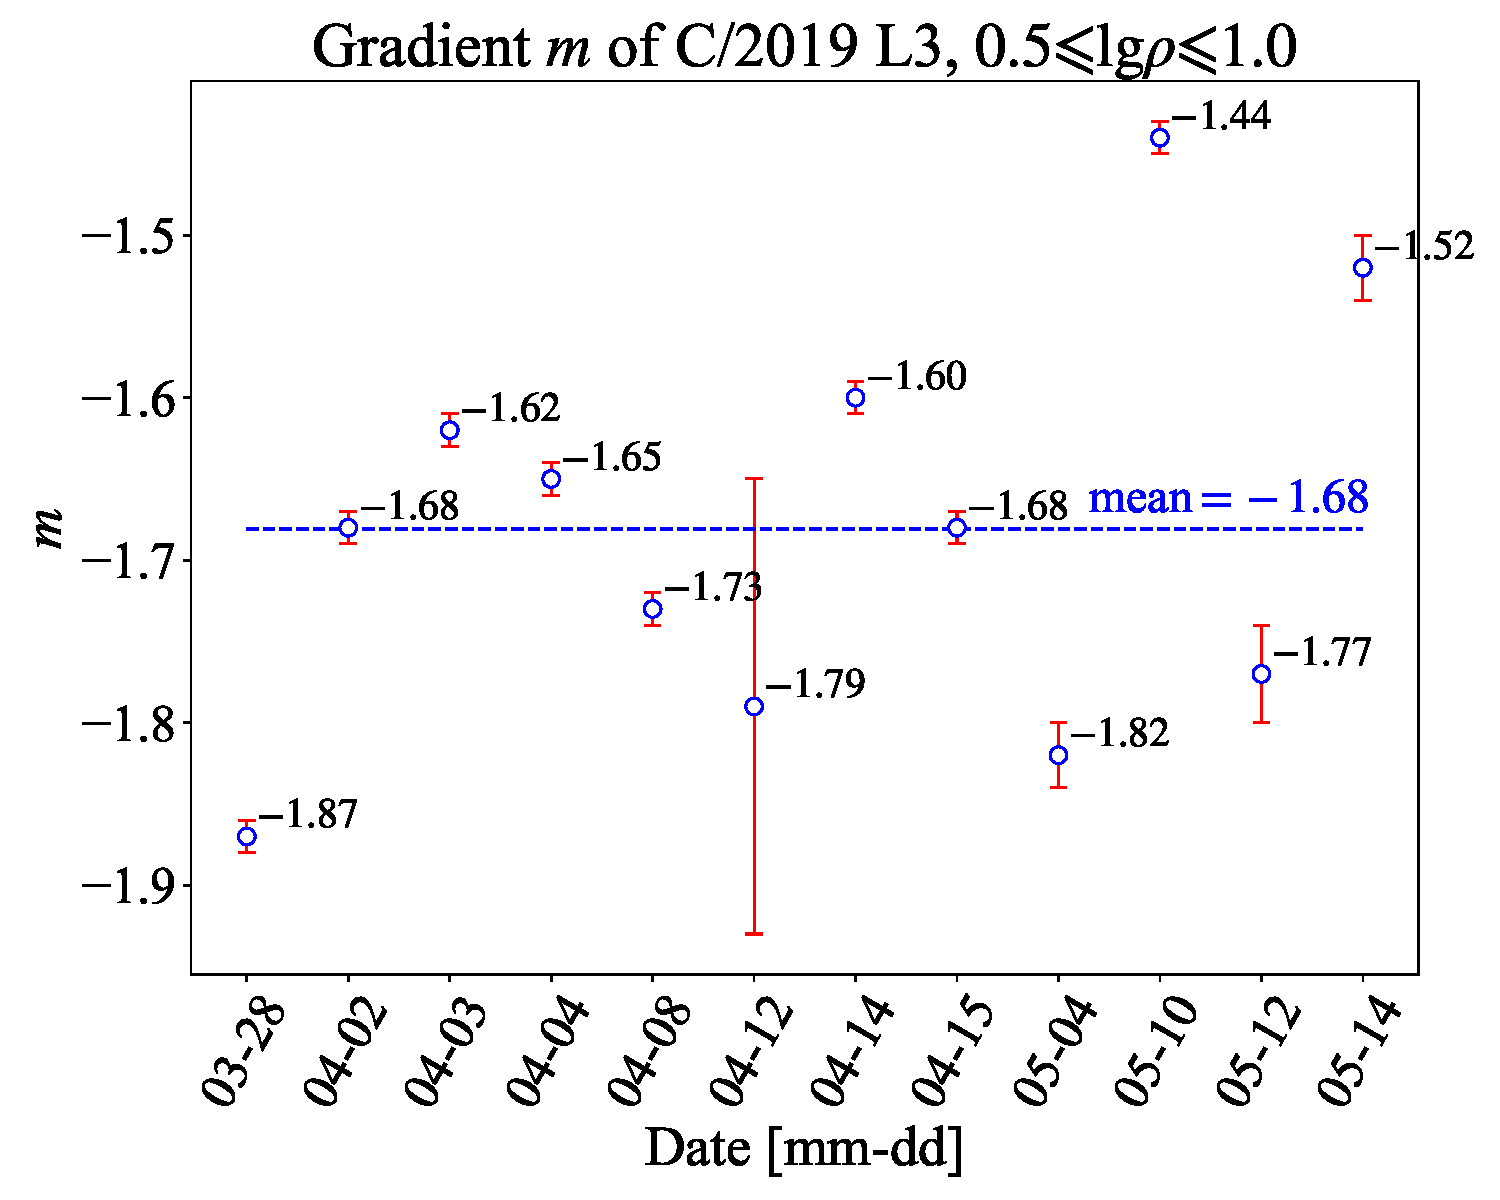
\includegraphics[width=\columnwidth]{sbp_m.pdf}
    \caption{The $m$ of R-band surface brightness of comet C/2019 L3 with date, blue dotted line is the averaged m. }
    \label{fig:sbp_m}
\end{figure}


\subsection{$Af\rho$}

The $Af\rho$ value introduced by \citet{ahearn_comet_1984}, where $A$ represents the gain albedo, $f$ the filling factor, and $\rho$ the aperture, is commonly used to indicate the dust production activity of comets. Usually it is expressed in \si{\cm} as equation (\ref{eq:afr}): 
\begin{equation}
    Af\rho = \frac{4 r^2 \Delta^2}{\rho} 10^{0.4(M_\odot - M_c)}, 
    \label{eq:afr}
\end{equation}
where $r$ is the heliocentric distance in \si{\astronomicalunit}, $\Delta$ the geocentric distance in \si{\km}, $\rho$ the aperture in \si{\km}, $M_\odot$ the absolute magnitude of the Sun (\si{\num{-26.13}} and \si{\num{-27.15}} for B and R filter, see \citealt{willmer_absolute_2018}), and $M_c$ the corresponding magnitude of comet under the aperture of $\rho$. 

Due to the phase darkening effect, it is necessary to adjust $Af\rho$ values at different phase angles to a specific angle. In this work, all observations were conducted at small phase angles, and we normalize the $Af\rho$ values to a phase angle of \ang{0} using equation (\ref{eq:a0frho}), as shown below:
\begin{equation}
    A(0)f\rho = \frac{A(\alpha)f\rho}{\phi(\alpha)}, \label{eq:a0frho}
\end{equation}
where $\alpha$ is the phase angle, and $\phi$ is the phase function. A composite phase function (see \citealt{schleicher_composition_2011, marcus_forward-scattering_2007}) suggested by D. Schleicher\footnote{\href{https://asteroid.lowell.edu/comet/dustphase.html}{https://asteroid.lowell.edu/comet/dustphase.html}} is suitable for adjustion in this work. The related dustphaseHM\_table\footnote{\href{https://asteroid.lowell.edu/comet/dustphaseHM_table.html}{https://asteroid.lowell.edu/comet/dustphaseHM\_table.html}} provides the phase function with phase angle in the $\ang{0} \leqslant \alpha \leqslant \ang{180}$ range, and we adopt cubic spline interpolation method on it to obtain unlisted values. 

Fig.~\ref{fig:Afrho} shows some part of the R-band $Af\rho$ profiles, and results for the maximum of $Af\rho$ and the aperture corresponding to this maximum are summarised in Table~\ref{tab:afrho}. When a comet possesses steady coma, its $Af\rho$ will be independent of aperture. In this paper, as is shown in Fig.~\ref{fig:Afrho}, that is not the case for comet C/2019 L3 or C/2020 P3, both of which reveal a steep increse in $Af\rho$ with the aperture $\rho$ near the comet center along with a smooth decrese with larger aperture. The increase results from usually the effect of seeing and observational circumstance, while the nonsteady dust emmission and possibly the fading or destruction of dust grain bring the decrease \citep{lara_behaviour_2003,tozzi_imaging_2003}.  
             
% 可选择相同日心距范围内的其他长周期彗星进行比较

%其中,$r$表示日心距(以AU为单位),$\Delta$表示地心距(以km为单位),$\rho$表示以km为单位的孔径,$M_\odot$和$M_c$分别表示太阳和彗星的星等。在比较不同彗星的活动性时,通常以$\rho = 10^4km$为基准比较它们$Af\rho$值的大小。

\begin{figure}
    \centering
    \subcaptionbox{}{
        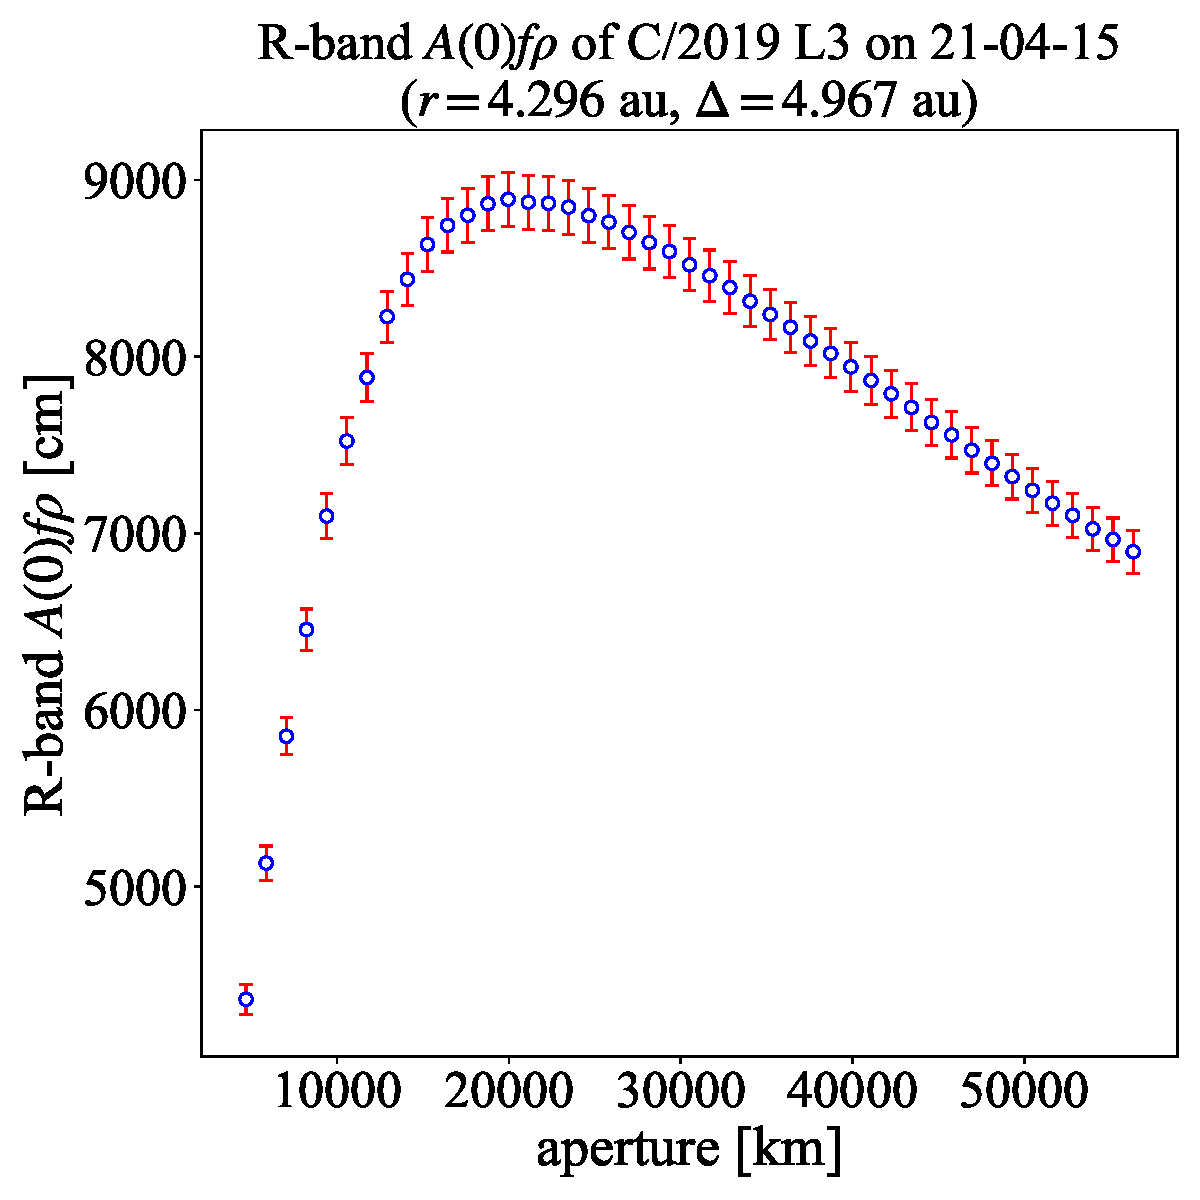
\includegraphics[width=.45\columnwidth]{R-Afrho-C2019L3-210415.pdf}
    }
    \subcaptionbox{}{
        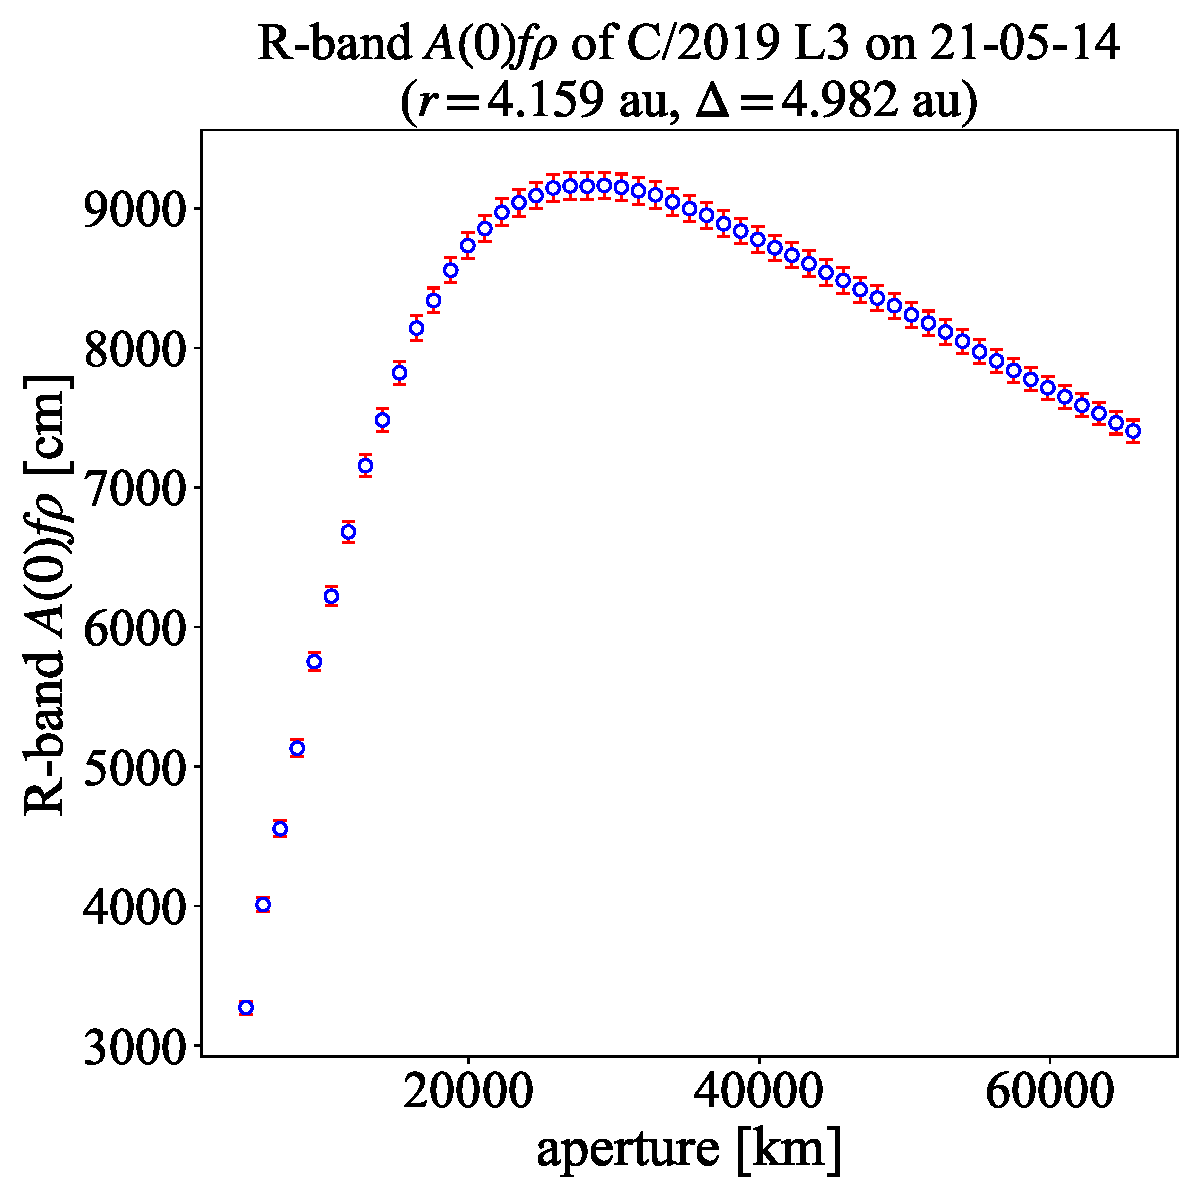
\includegraphics[width=.45\columnwidth]{R-Afrho-C2019L3-210514.pdf}
    }

    \subcaptionbox{}{
        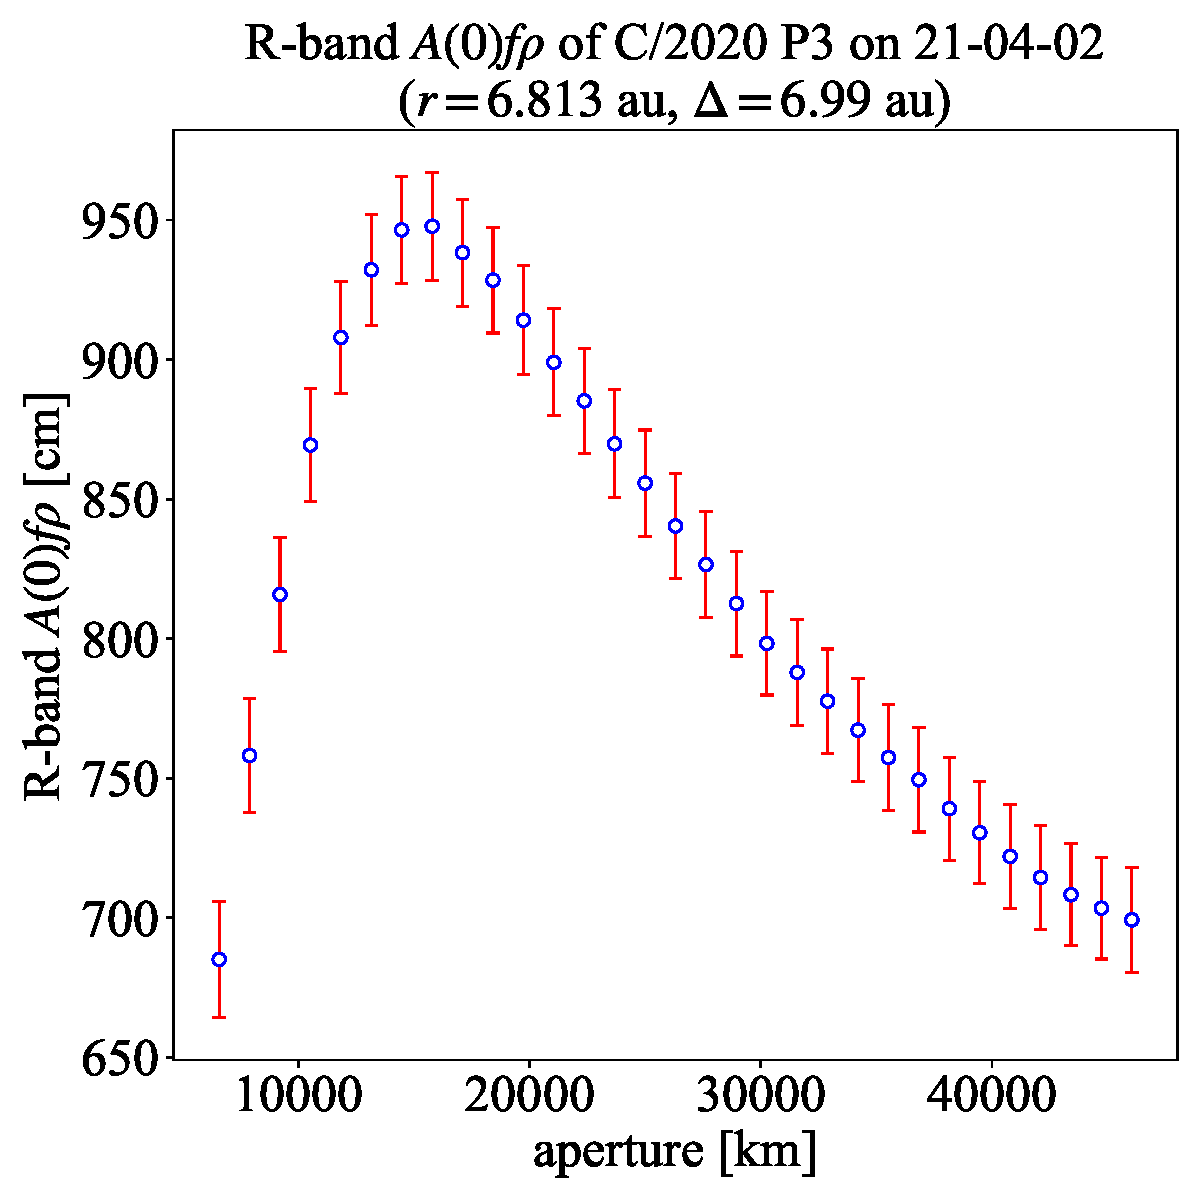
\includegraphics[width=.45\columnwidth]{R-Afrho-C2020P3-210402.pdf}
    }
    \subcaptionbox{}{
        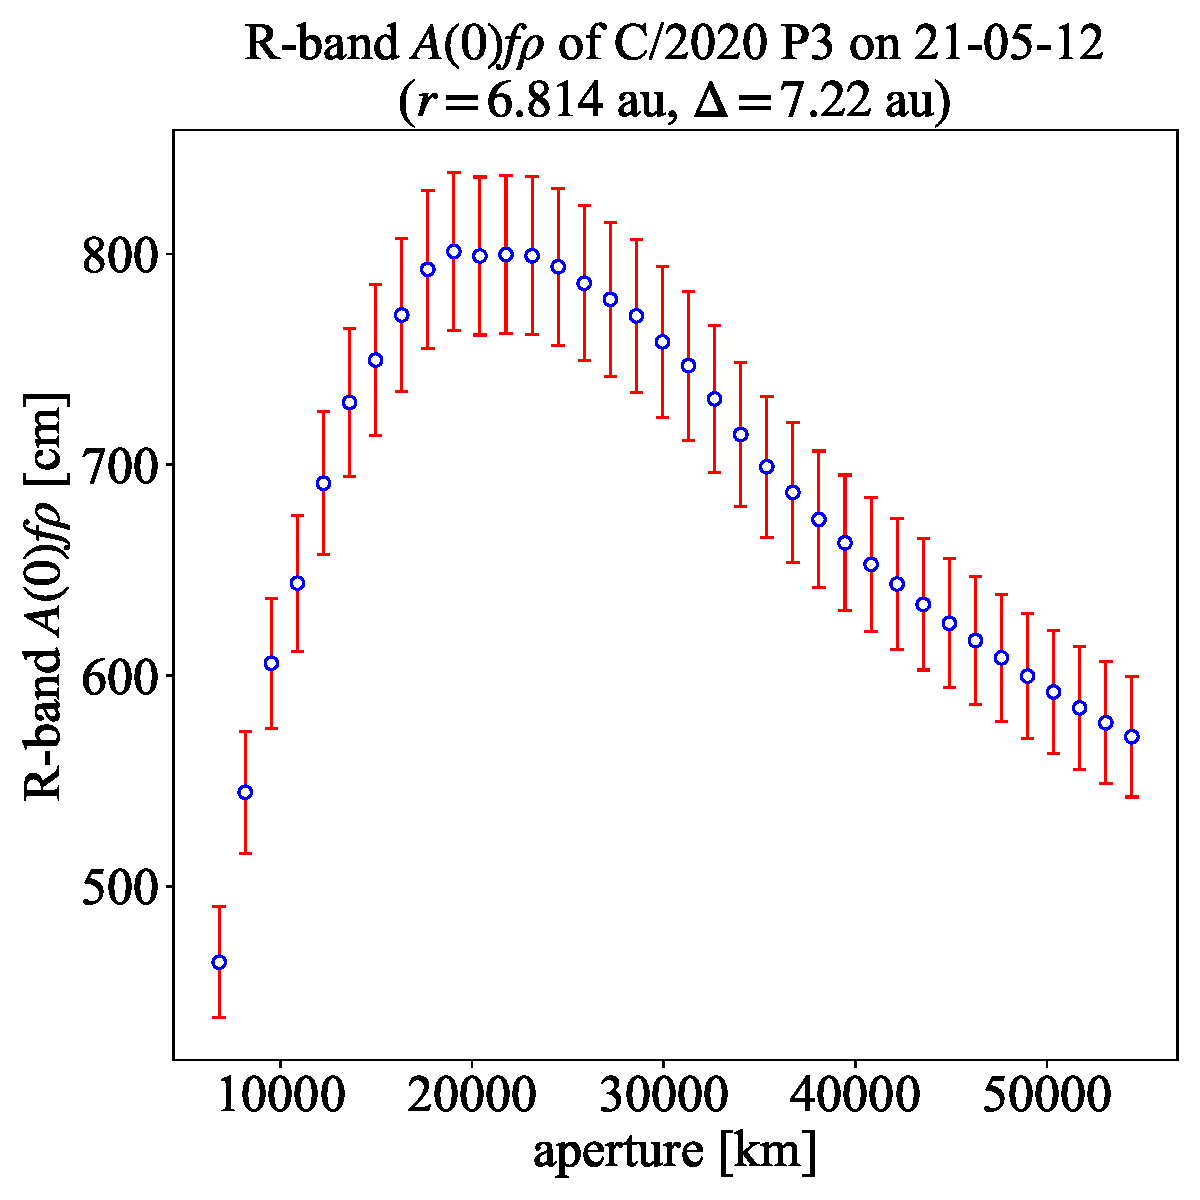
\includegraphics[width=.45\columnwidth]{R-Afrho-C2020P3-210512.pdf}
    }
    \caption{R-band $Af\rho$ of comet C/2019 L3 and C/2020 P3. }
    \label{fig:Afrho}
\end{figure}

% 统一至20000km?
% Afrho
\begin{table}
    \centering
    \caption{$Af\rho$ values for comet C/2019 L3 and C/2020 P3. }\label{tab:afrho}
    \begin{threeparttable}
        \resizebox{\linewidth}{!}{
        \begin{tabular}{cccc}
            \toprule
            Observation Time & $Af\rho$ ($\rho =$ \SI{e4}{\km}) & $Af\rho_{max}$ [\si{\cm}] & $\rho_{max}$ [\si{\km}]\\
            \midrule
            \multicolumn{4}{l}{\textbf{C/2019 L3}} \\
            2021-03-28.729 & \num{13611 +- 1874} & \num{13615 +- 1875} & \num{10373} \\
            2021-04-02.739 & \num{9332 +- 539} & \num{10748 +- 618} & \num{20930} \\
            2021-04-03.719 & \num{7959 +- 143} & \num{10869 +- 729} & \num{22093} \\
            2021-04-04.691 & \num{6220 +- 69} & \num{9003 +- 114} & \num{20930} \\
            2021-04-08.691 & \num{8985 +- 603} & \num{8700 +- 110} & \num{19860} \\
            2021-04-12.724 & \num{7911 +- 102} & \num{7410 +- 269} & \num{29343} \\
            2021-04-14.702 & \num{7320 +- 95} & \num{8268 +- 133} & \num{25822} \\
            2021-04-15.714 & \num{5043 +- 244} & \num{8891 +- 154} & \num{19953} \\
            2021-05-04.736 & \num{5943 +- 96} & \num{8320 +- 340} & \num{29365} \\
            2021-05-10.735 & \num{7523 +- 134} & \num{8787 +- 205} & \num{29343} \\
            2021-05-12.724 & \num{5701 +- 236} & \num{9590 +- 157} & \num{21127} \\
            2021-05-14.721 & \num{6356 +- 152} & \num{9164 +- 95} & \num{29343} \\
            \multicolumn{4}{l}{\textbf{C/2020 P3}} \\
            2021-04-02.775 & \num{869 +- 20} & \num{948 +- 19} & \num{15789} \\
            2021-05-11.744 & \num{708 +- 17} & \num{848 +- 17} & \num{19048} \\
            2021-05-12.749 & \num{606 +- 31} & \num{801 +- 38} & \num{19048} \\
            \bottomrule
        \end{tabular}
        }
    \end{threeparttable}
\end{table}


\begin{comment}
\begin{figure}[h]
    %\centering
    %\begin{subfigure}{0.5\textwidth}
    \ContinuedFloat
        \subcaptionbox{}{
            \includegraphics[width=.48\linewidth]{Afrho_C2019_4.pdf}
        }
        \subcaptionbox{}{
            \includegraphics[width=.48\linewidth]{Afrho_C2019_5.pdf}
        }

        \subcaptionbox{}{
            \includegraphics[width=.48\linewidth]{Afrho_C2019_6.pdf}
        }
        \subcaptionbox{}{
            \includegraphics[width=.48\linewidth]{Afrho_C2019_7.pdf}
        }
    %\label{fig:first}
    %\end{subfigure}
    \caption{(续)$Af\rho$ of comet C/2019 L3 and C/2020 P3.}
\end{figure}
\end{comment}

\begin{comment}
\begin{figure}[h]
    %\centering
    %\begin{subfigure}{0.5\textwidth}
    
        \subcaptionbox{}{
            \includegraphics[width=.48\linewidth]{Afrho_C2019_0.pdf}
        }
        \subcaptionbox{}{
            \includegraphics[width=.48\linewidth]{Afrho_C2019_1.pdf}
        }

    %\label{fig:first}
    %\end{subfigure}
    \caption{$Af\rho$ of comet C/2019 L3 and C/2020 P3.}
    \label{fig:Afrhomax}
\end{figure}
\begin{figure}[h]
    \ContinuedFloat
    %\centering
    %\begin{subfigure}{0.5\textwidth}
    
        \subcaptionbox{}{
            \includegraphics[width=.48\linewidth]{Afrho_C2019_2.pdf}
        }
        \subcaptionbox{}{
            \includegraphics[width=.48\linewidth]{Afrho_C2019_3.pdf}
        }

    %\label{fig:first}
    %\end{subfigure}
    \caption{$Af\rho$ of comet C/2019 L3 and C/2020 P3.}
    %\label{fig:figures}
\end{figure}
\begin{figure}[h]
    \ContinuedFloat
    %\centering
    %\begin{subfigure}{0.5\textwidth}
    
        \subcaptionbox{}{
            \includegraphics[width=.48\linewidth]{Afrho_C2019_4.pdf}
        }
        \subcaptionbox{}{
            \includegraphics[width=.48\linewidth]{Afrho_C2019_5.pdf}
        }

    %\label{fig:first}
    %\end{subfigure}
    \caption{$Af\rho$ of comet C/2019 L3 and C/2020 P3.}
    %\label{fig:figures}
\end{figure}
\begin{figure}[h]
    \ContinuedFloat
    %\centering
    %\begin{subfigure}{0.5\textwidth}
    
        \subcaptionbox{}{
            \includegraphics[width=.48\linewidth]{Afrho_C2019_6.pdf}
        }
        \subcaptionbox{}{
            \includegraphics[width=.48\linewidth]{Afrho_C2019_7.pdf}
        }

    %\label{fig:afr}
    %\end{subfigure}
    \caption{$Af\rho$ of comet C/2019 L3 and C/2020 P3.}
    %\label{fig:Afrhomax}
\end{figure}
\begin{figure}[h]
    \ContinuedFloat
    %\centering
    %\begin{subfigure}{0.5\textwidth}
    
        \subcaptionbox{}{
            \includegraphics[width=.48\linewidth]{Afrho_C2019_8.pdf}
        }
        \subcaptionbox{}{
            \includegraphics[width=.48\linewidth]{Afrho_C2019_9.pdf}
        }

    %\label{fig:first}
    %\end{subfigure}
    \caption{$Af\rho$ of comet C/2019 L3 and C/2020 P3.}
    %\label{fig:figures}
\end{figure}
\begin{figure}[h]
    \ContinuedFloat
    %\centering
    %\begin{subfigure}{0.5\textwidth}
    
        \subcaptionbox{}{
            \includegraphics[width=.48\linewidth]{Afrho_C2019_10.pdf}
        }
        \subcaptionbox{}{
            \includegraphics[width=.48\linewidth]{Afrho_C2019_11.pdf}
        }

    %\label{fig:first}
    %\end{subfigure}
    \caption{$Af\rho$ of comet C/2019 L3 and C/2020 P3.}
    %\label{fig:Afrhomax}
\end{figure}
\begin{figure}[h]
    \ContinuedFloat
    %\centering
    %\begin{subfigure}{0.5\textwidth}
    
        \subcaptionbox{}{
            \includegraphics[width=.48\linewidth]{Afrho_C2020_0.pdf}
        }
        \subcaptionbox{}{
            \includegraphics[width=.48\linewidth]{Afrho_C2020_1.pdf}
        }

    %\label{fig:first}
    %\end{subfigure}
    \caption{$Af\rho$ of comet C/2019 L3 and C/2020 P3.}
    %\label{fig:Afrhomax}
\end{figure}
\begin{figure}[h]
    \ContinuedFloat
    %\centering
    %\begin{subfigure}{0.5\textwidth}
    
        \subcaptionbox{}{
            \includegraphics[width=.48\linewidth]{Afrho_C2020_2.pdf}
        }
        \subcaptionbox{}{
            \includegraphics[width=.48\linewidth]{Afrho_C2020_3.pdf}
        }

    %\label{fig:first}
    %\end{subfigure}
    \caption{$Af\rho$ of comet C/2019 L3 and C/2020 P3.}
    %\label{fig:Afrhomax}
\end{figure}
\end{comment}



\begin{comment}
% Afrho_max
\begin{table}[!htbp]
    \centering
    \caption{Review of images: C/2019 L3 and C/2020 P3}\label{tab:c2019andc2020}
    \tiny
    \begin{threeparttable}
        \begin{tabular}{cccc}
            \toprule
            Observation Date & $Afrho_{max}$ & $Af\rho_{err}$ & $\rho_{max}$ \\
            \midrule
            \multicolumn{8}{c}{\textbf{C/2019 L3}} \\
            2021-03-28 & 4.385 & 4.916 & 10.4 \\
            2021-04-02 & 4.360 & 4.933 & 10.1 \\
            2021-04-03 & 4.355 & 4.936 & 10.1 \\
            2021-04-04 & 4.350 & 4.939 & 10.0 \\
            2021-04-08 & 4.331 & 4.950 & 9.7  \\
            2021-04-12 & 4.311 & 4.960 & 9.5  \\
            2021-04-14 & 4.301 & 4.965 & 9.3  \\
            2021-04-15 & 4.296 & 4.967 & 9.3  \\
            2021-05-04 & 4.205 & 4.987 & 8.0  \\
            2021-05-10 & 4.177 & 4.985 & 7.6  \\
            2021-05-12 & 4.168 & 4.984 & 7.5  \\
            2021-05-14 & 4.159 & 4.982 & 7.4  \\

            \multicolumn{8}{c}{\textbf{C/2020 P3}} \\
            2021-03-28 & 6.956 & 6.814 & 8.2 \\
            2021-04-02 & 6.990 & 6.813 & 8.2 \\
            2021-05-11 & 4.205 & 7.216 & 6.814  \\
            2021-05-12 & 4.159 & 7.221 & 6.814  \\
            \bottomrule
        \end{tabular}
        \begin{tablenotes}
            \item[1] heliocentric distance
            \item[2] geocentric distance
            \item[3] phase angle
        \end{tablenotes}
    \end{threeparttable}
\end{table}
\end{comment}


\begin{comment}
%%%%%%%% Continue figures %%%%%%%%
        
\begin{figure}[h]
    \ContinuedFloat
    
    \begin{subfigure}{\textwidth}
    \centering
    \includegraphics[width=0.7\textwidth]{Afrho_C2019_1.pdf}
    \caption{Second subfigure.}
    \label{fig:second}
    \end{subfigure}
    \begin{subfigure}{\textwidth}
    \centering
    \includegraphics[width=0.7\textwidth]{Afrho_C2019_2.pdf}
    \caption{Third subfigure.}
    \label{fig:third}
    \end{subfigure}
    
    \caption{Page breaks and subfigures.}
    \label{fig:figures}
    
\end{figure}
\end{comment}

%平均尘埃生成率的计算如~\autoref{eq:dpr}~所示:

%\begin{equation}
%    \frac{\mathrm{d}M}{\mathrm{d}t} = \frac{4}{3} \frac{\rho \bar{a} C_e}{\tau_r}
%    \label{eq:dpr}
%\end{equation}

%式中,$\rho$是喷射的固体物质的体积密度,$\bar{a}$是颗粒的加权平均半径,$C_e$是测光孔径下的散射截面,$\tau_r$是尘埃在孔径中的停留时间。

\subsection{Coma Colors}

The photometric results in Table~\ref{tab:bvr} also summarises the color index of the two comets. 
The average colors for C/2019 L3 are as follows: 
$\langle \mathrm{B} - \mathrm{V} \rangle = \num{0.75 +- 0.06}$, 
$\langle \mathrm{V} - \mathrm{R} \rangle = \num{0.27 +- 0.05}$, and 
$\langle \mathrm{R} - \mathrm{I} \rangle = \num{0.22 +- 0.05}$. 
On the other hand, the average colors for C/2020 P3 are 
$\langle \mathrm{B} - \mathrm{V} \rangle = \num{0.95 +- 0.07}$, 
$\langle \mathrm{V} - \mathrm{R} \rangle = \num{0.29 +- 0.05}$, and 
$\langle \mathrm{R} - \mathrm{I} \rangle = \num{0.21 +- 0.05}$. 
Moreover, in order to indicate how the scattered color of the dusty coma varies with wavelengths, the reddening $\mathcal{R}$ (or normalized color) \citep{jewitt_cometary_1986, lara_behaviour_2003, mazzotta_epifani_dust_2011, shi_ccd_2015} is calculated in \si{\percent/\kilo\angstrom}, with the formula given as equation (\ref{eq:red}): 
\begin{equation}
\mathcal{R} = \frac{2}{Af\rho_1 + Af\rho_2} \frac{Af\rho_2 - Af\rho_1}{\lambda_2 - \lambda_1}, 
\label{eq:red}
\end{equation}
where $\lambda_1$ and $\lambda_2$ are the central wavelengths of the filters in \si{\nm} (respectively the centers of B and R filters, {\SI{440}{\nm}} and {\SI{658}{\nm}}). With this parameter it is convenient to indicate the percentage of change in the strength of the continuum per {\SI{1000}{\angstrom}}. The results of dust reddening are summarised in Table~\ref{tab:reddening}. In order to avoid the possible effects from background residuals, it is calculated with aperture of {\SI{2e4}{\km}}. 

For comet C/2019 L3, the reddening undergoes significant variations over time, from positive value {\SI{13.75 +- 1.07}{\percent/\kilo\angstrom}} on \DTMdate{2021-3-28} to negative value {\SI{-15.69 +- 0.37}{\percent/\kilo\angstrom}} on \DTMdate{2021-4-12}. We plot the reddening as a function of date in Fig.~\ref{fig:reddening}, and the averaged value \num{0.94 +- 0.23} is marked as a horizontal blue dotted line. For comet C/2020 P3, only on \DTMdate{2021-5-12} is its observational data sufficient for the calcltaion of reddening with a result of {\SI{-6.65 +- 0.01}{\percent/\kilo\angstrom}}. 

\begin{table}
    \centering
    \caption{Reddening of comet C/2019 L3 and C/2020 P3 with $\rho = $ \SI{2e4}{\km} }\label{tab:reddening}
    \begin{threeparttable}
        \resizebox{\linewidth}{!}{
        \begin{tabular}{cccc}
            \toprule
            Observation Time & B-band $Af\rho$ & R-band $Af\rho$ & reddening [\si{\%/\kilo\angstrom}]\\
            \midrule
            \multicolumn{4}{l}{\textbf{C/2019 L3}} \\
            2021-03-28.729 & \num{9472 +- 753} & \num{12811 +- 1764} & \num{13.75 +- 1.07}\\
            2021-04-02.739 & \num{8763 +- 806} & \num{10719 +- 617} & \num{9.21 +- 0.50}\\
            2021-04-03.719 & \num{9886 +- 274} & \num{9538 +- 156} & \num{-1.65 +- 0.03}\\
            2021-04-04.691 & \num{9501 +- 343} & \num{8734 +- 93} & \num{-3.86 +- 0.07}\\
            2021-04-08.691 & \num{9288 +- 402} & \num{10797 +- 725} & \num{6.89 +- 0.27}\\
            2021-04-12.724 & \num{12683 +- 602} & \num{8979 +- 113} & \num{-15.69 +- 0.37}\\
            2021-04-14.702 & \num{8809 +- 382} & \num{8700 +- 110} & \num{-0.57 +- 0.01}\\
            2021-04-15.714 & \num{6077 +- 283} & \num{7173 +- 271} & \num{7.59 +- 0.23}\\
            2021-05-04.736 & \num{7724 +- 264} & \num{8065 +- 130} & \num{1.98 +- 0.04}\\
            2021-05-10.735 & \num{9030 +- 285} & \num{8891 +- 154} & \num{-0.71 +- 0.01}\\
            2021-05-12.724 & \num{9044 +- 336} & \num{7958 +- 326} & \num{-5.86 +- 0.16}\\
            2021-05-14.721 & \num{8428 +- 258} & \num{8475 +- 199} & \num{0.25 +- 0.00}\\
            \multicolumn{4}{l}{\textbf{C/2020 P3}} \\
            2021-05-12.749 & \num{934 +- 74} & \num{799 +- 37} & \num{-6.65 +- 0.01}\\
            \bottomrule
        \end{tabular}
        }
    \end{threeparttable}
\end{table}

\begin{figure}
    \centering
    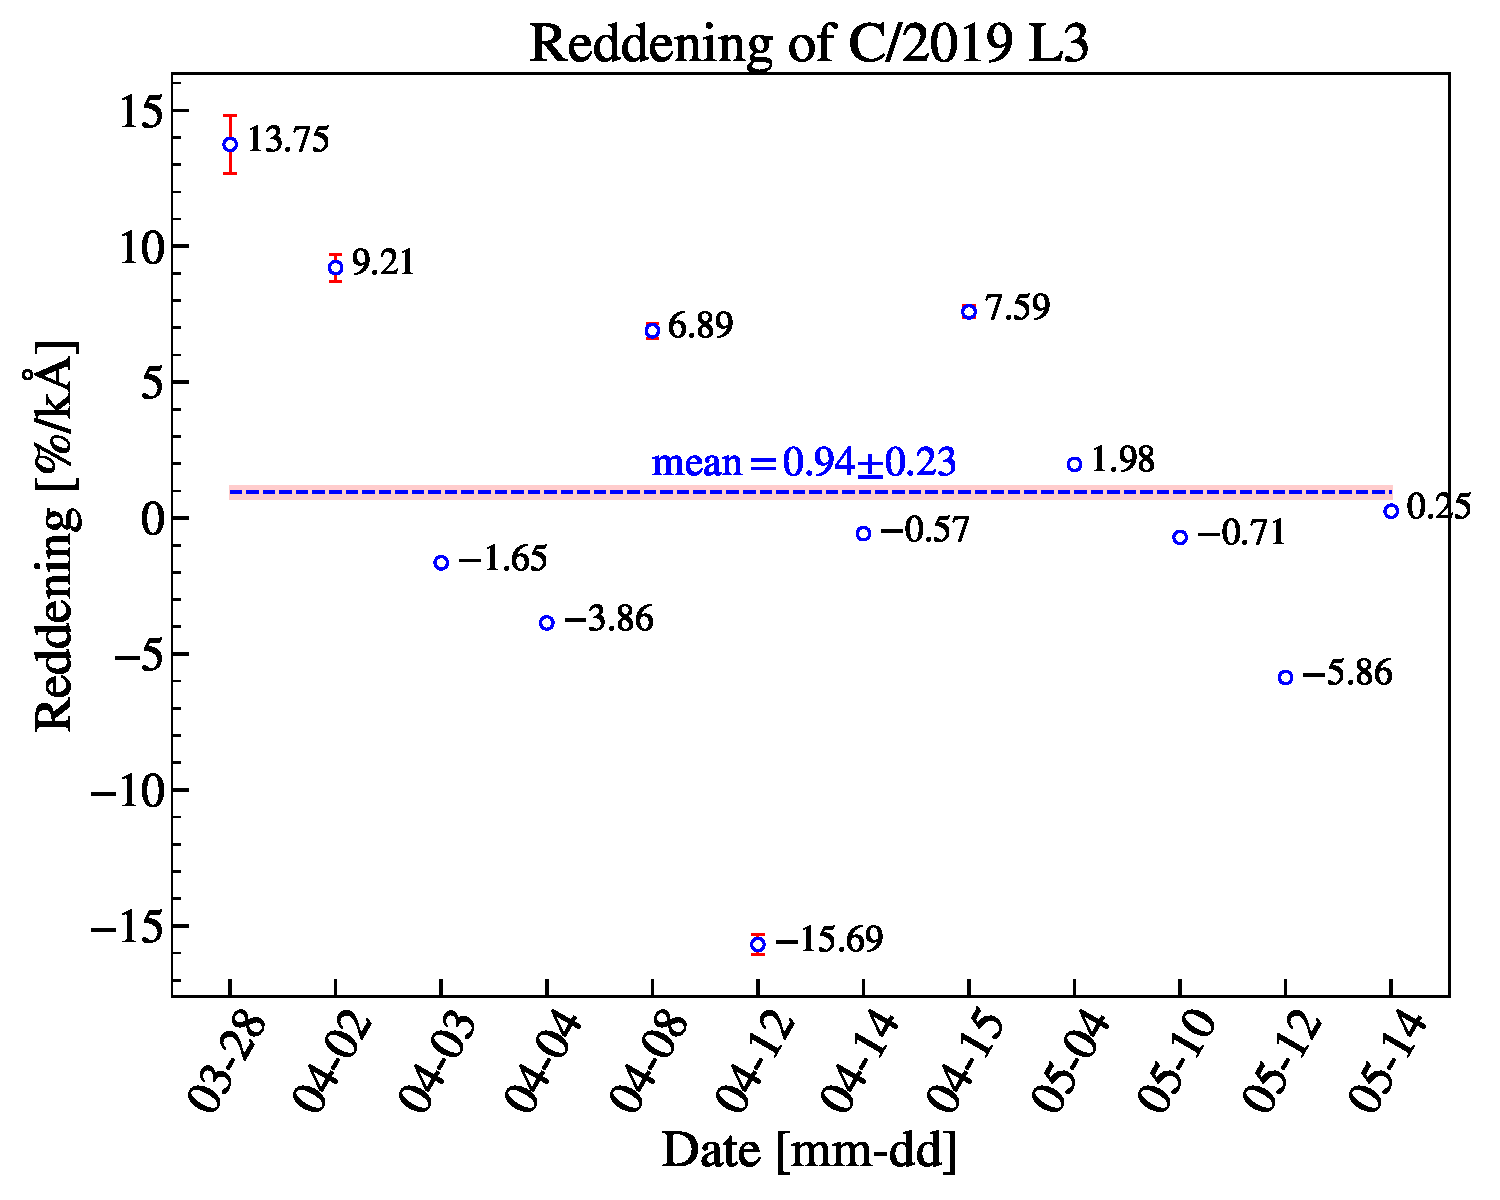
\includegraphics[width=\columnwidth]{reddening.pdf}
    \caption{The reddening of comet C/2019 L3 with date, blue dotted line is the averaged reddening. }\label{fig:reddening}
\end{figure}


\section{Discussion and Conclusion}\label{sec:dis}


% From \autoref{tab:afrho} we can conclude that the comet C/2019 L3 is very active due to its high $A(0)f\rho$ values during the observational run, while C/2020 P3 is less active since its $A(0)f\rho$ values are only about {\SI{10}{\percent}} of that of C/2019 L3. 
Comparing $A(0)f\rho$ values with that of other LPCs, just as Fig.~\ref{fig:afrho-ref} shown, C/2019 L3 is very active at heliocentric distance of $\thicksim${\qty{4}{\astronomicalunit}}, and C/2020 P3 is moderately active at heliocentric distance of $\thicksim${\qty{7}{\astronomicalunit}}. 
Moreover, % 在此只写活动性显现出异常, 不作过度猜测
it can be seen from Fig.~\ref{fig:a0frho-c2019} that during the observation period, the R-band $A(0)f\rho$ values of comet C/2019 L3, measured at an aperture of {\SI{e4}{\km}}, showed a trend of initially decreasing followed by an increase. This could be attributed to a previous outburst, followed by a gradual increase in activity as it approaches perihelion. 
On the other hand, 
the BC-band $A(0)f\rho$ value of C/2019 L3 up to \SI{24710 +- 125}{\cm} on \DTMdate{2022-1-19} posted on The Astronomer's Telegram\footnote{\href{https://www.astronomerstelegram.org/?read=15186}{https://www.astronomerstelegram.org/?read=15186}}, with heliocentric distance $r = \SI{3.56}{\astronomicalunit}$ and geocentric distance $\Delta = \SI{2.61}{\astronomicalunit}$, indicates that C/2019 L3 appears very active near the perihelion. 


% 与其他LPC比较,相位角均校正至0
\begin{figure}
    \centering
    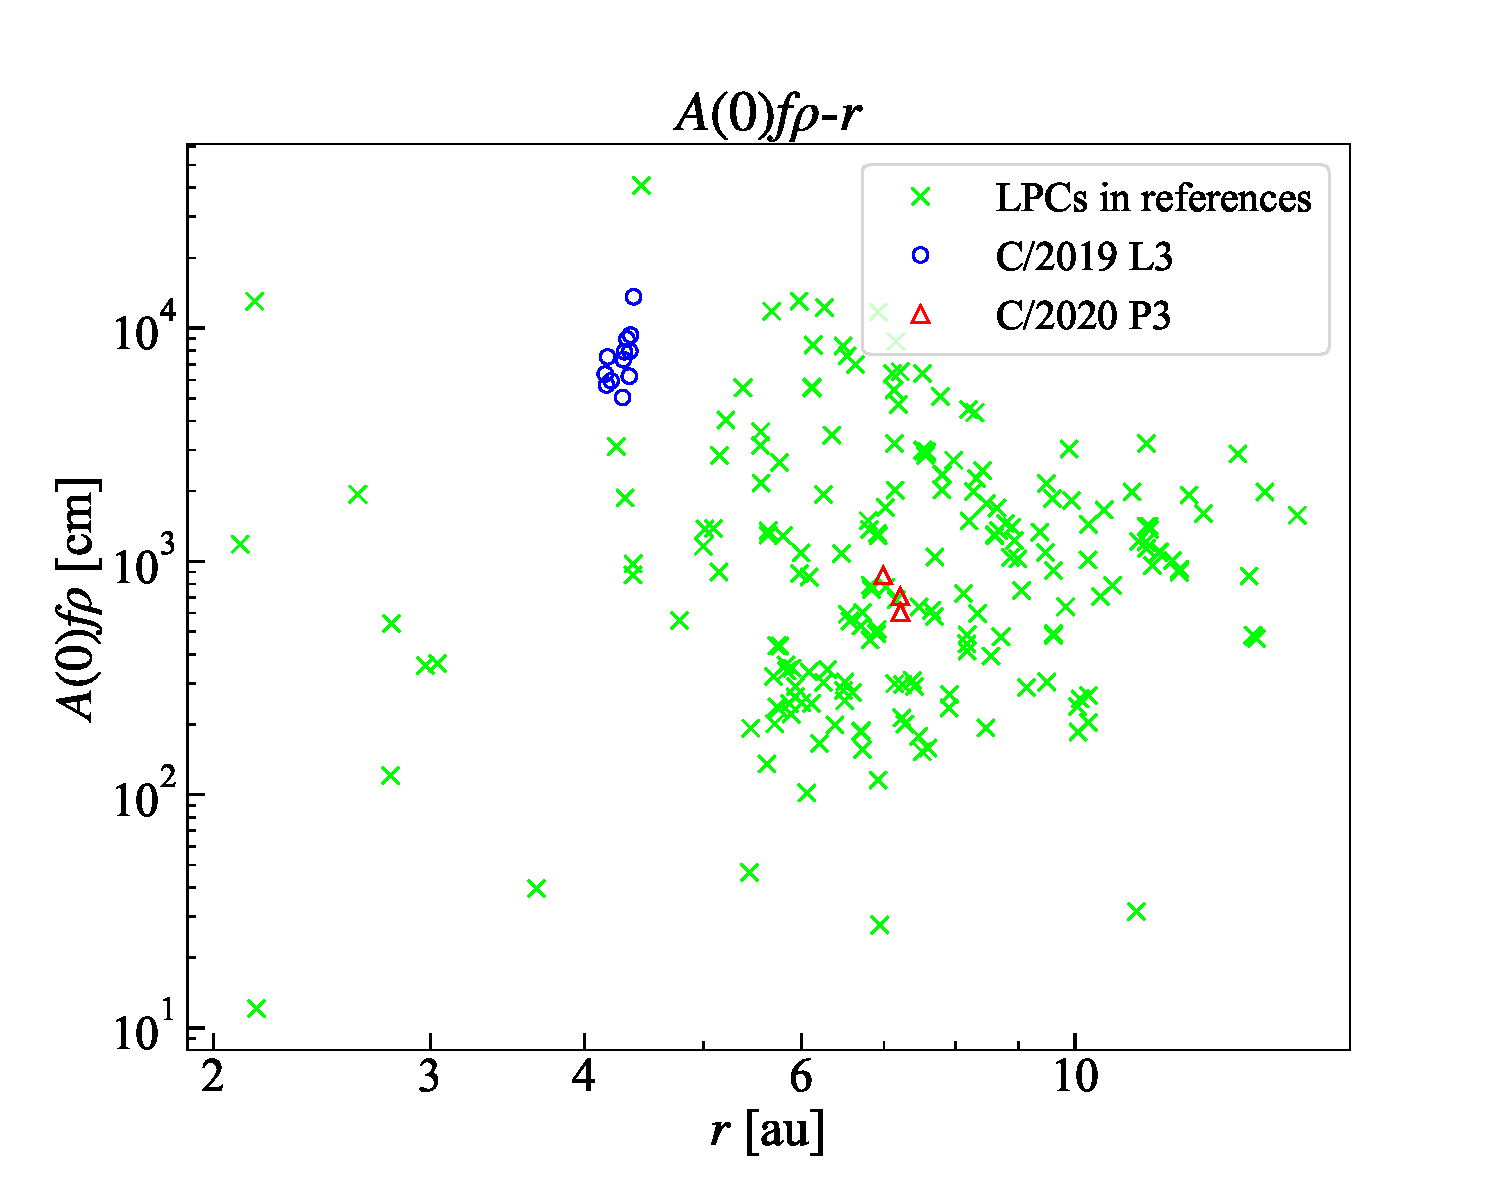
\includegraphics[width=\columnwidth]{a0frho-r.pdf}
    \caption{$A(0)f\rho$ values measured in this work compared with that of other LPCs in  literature by \citet{mazzotta_epifani_observational_2014}, \citet{garcia_photometry_2021}, \citet{garcia_observational_2020}, \citet{rousselot_monitoring_2014}, \citet{meech_activity_2009}, \citet{sarneczky_activity_2016}, \citet{solontoi_ensemble_2012}, and \citet{szabo_spectrophotometry_2002}. All data have been adjusted to phase angle \ang{0}. }\label{fig:afrho-ref}
\end{figure}% data amount error

\begin{figure}
    \centering
    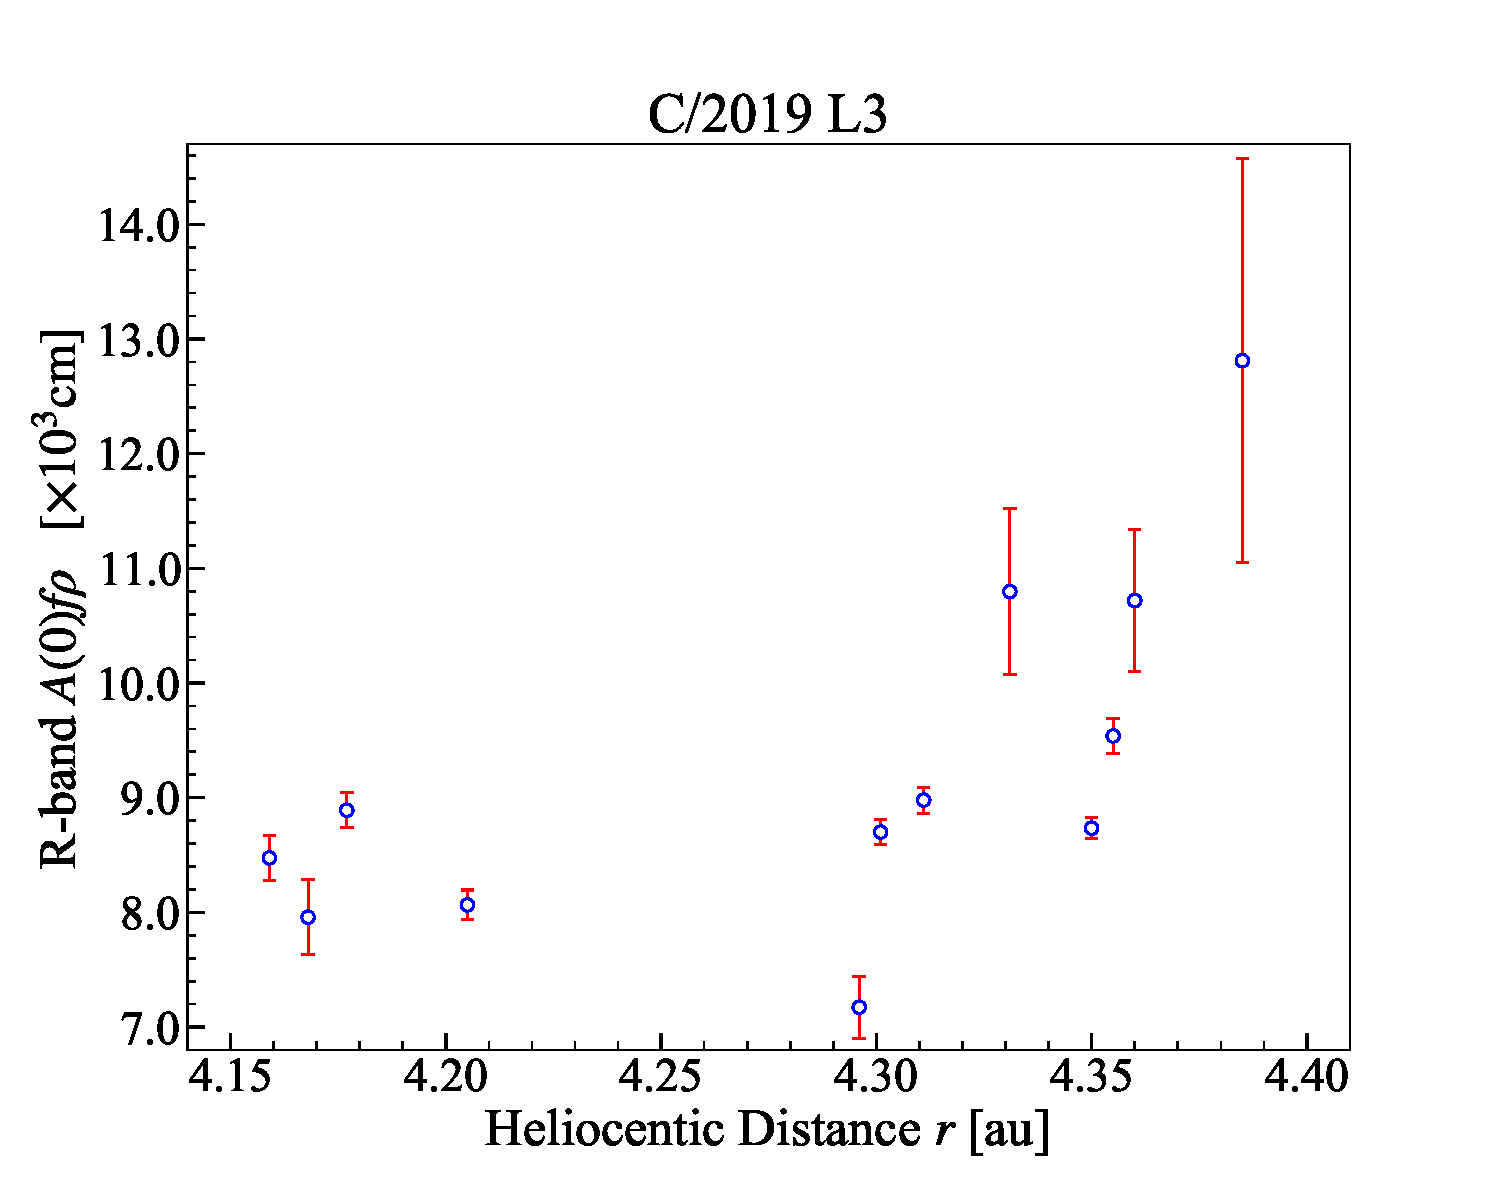
\includegraphics[width=\columnwidth]{a0frho-r-C2019L3-new.pdf}
    \caption{R-band $A(0)f\rho$ values of C/2019 L3 as a function of heliocentric distance. }\label{fig:a0frho-c2019}
\end{figure}

According to the study by \cite{ramirez_ubvric_2012}, the solar colors are as follows: 
${(\mathrm{B} - \mathrm{V})}_{\odot} = \num{0.653 +- 0.005}$, 
${(\mathrm{V} - \mathrm{R})}_{\odot} = \num{0.352 +- 0.007}$, and 
${(\mathrm{R} - \mathrm{I})}_{\odot} = \num{0.350 +- 0.009}$. 
The average color indices of two Long-period comets and three dynamically new comets were calculated by \cite{meech_activity_2009} to be 
$\langle \mathrm{B} - \mathrm{V} \rangle = \num{0.76 +- 0.01}$ and 
$\langle \mathrm{V} - \mathrm{R} \rangle = \num{0.43 +- 0.01}$, 
with their heliocentric distances ranging from \SIrange{5.8}{14.0}{\astronomicalunit}. 
\cite{solontoi_ensemble_2012} studied six Long-period comets within \SI{5}{\astronomicalunit} of the Sun and obtained the average color indices of 
$\langle \mathrm{B} - \mathrm{V} \rangle = \num{0.687 +- 0.005}$ and 
$\langle \mathrm{V} - \mathrm{R} \rangle = \num{0.443 +- 0.003}$. 
\cite{jewittCOLORSYSTEMATICSCOMETS2015} investigated Long-period comets with large range of heliocentric distances (\SIrange{1.875}{17.982}{\astronomicalunit}), and the average color indices were found to be 
$\langle \mathrm{B} - \mathrm{V} \rangle = \num{0.78 +- 0.02}$, 
$\langle \mathrm{V} - \mathrm{R} \rangle = \num{0.47 +- 0.02}$, and 
$\langle \mathrm{R} - \mathrm{I} \rangle = \num{0.42 +- 0.03}$. 


Fig.~\ref{fig:color-color} is the $\langle \mathrm{B}-\mathrm{V} \rangle$ versus $\langle \mathrm{V}-\mathrm{R} \rangle$ plot of C/2019 L3, C/2020 P3 and other LPCs. 
The color index of the Sun \citep{ramirez_ubvric_2012} is marked as a red circle with dot. 
As we can see, the $\langle \mathrm{B} - \mathrm{V} \rangle$ colors of two comets are redder than the Sun, while the $\langle \mathrm{V} - \mathrm{R} \rangle$ colors of them are bluer than the Sun. 
Compared with LPCs in other works, the $\langle \mathrm{B} - \mathrm{V} \rangle$ color of C/2019 L3 is consistent with them, while the $\langle \mathrm{V} - \mathrm{R} \rangle$ color of C/2019 L3 is significantly bluer than them. For C/2020 P3, the $\langle \mathrm{B} - \mathrm{V} \rangle$ color is redder while the $\langle \mathrm{V} - \mathrm{R} \rangle$ color is bluer. 
In general, the color indices of the two LPCs studied in this work differ from those of other LPCs. 


% V-R随日心距呈现变蓝的趋势, 在4au左右CO2的升华作用较明显, 因此, C/2019 L3的活动性可能是由于CO2的升华导致

\begin{figure}
    \centering
    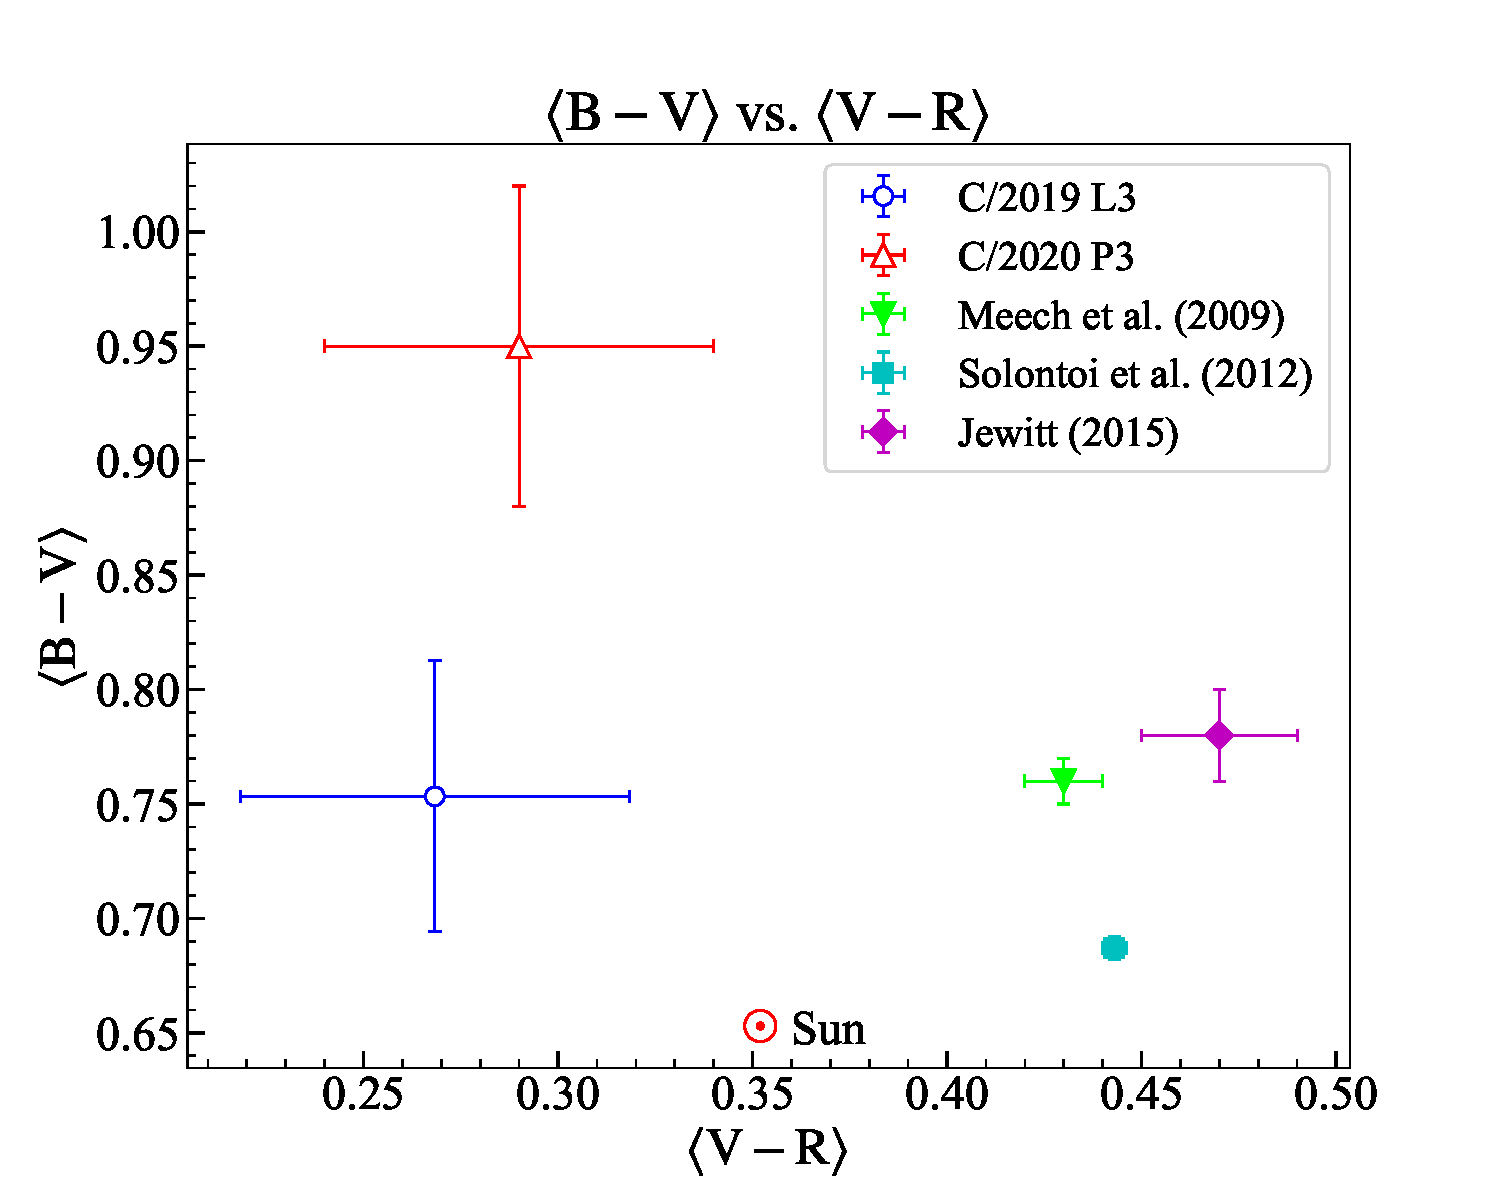
\includegraphics[width=\linewidth]{color-color.pdf}
    \caption{Color indices $\langle \mathrm{B-V} \rangle$ versus $\langle \mathrm{V-R} \rangle$ plot of Long-period comets}\label{fig:color-color}
\end{figure}

In summary, we present the observational results of comets C/2019 L3 and C/2020 P3. The conclusions are as follows: 
\begin{enumerate}
    \item For comet C/2019 L3, A fan-shape structure can be observed in the northeast direction. This feature is visible in both V and R filters. 
    \item The average gradient value  of the surface brightness profile of comet C/2019 L3 is \num{-1.66}, suggesting a nonsteady coma. 
    \item The R-band $A(0)f\rho$ values of C/2019 L3 range from {\qty{5043 +- 244}{\cm}} to {\qty{13611 +- 1874}{\cm}}, and those of C/2020 P3 range from {\qty{606 +- 31}{\cm}} to {\qty{869 +- 20}{\cm}}. Compared to other works, the $A(0)f\rho$ of C/2019 L3 is relatively high at $\thicksim${\qty{4}{\astronomicalunit}}, while that of C/2020 P3 is moderate at $\thicksim${\SI{7}{\astronomicalunit}}. The R-band $A(0)f\rho$ values of C/2019 L3 tend to decrease first and then increase, so it is possible that comet C/2019 L3 experienced an outburst event in the past, and it was still active after this stage. 
    \item The average colors for C/2019 L3 are  
        $\langle \mathrm{B-V} \rangle = \num{0.75 +- 0.06}$, 
        $\langle \mathrm{V-R} \rangle = \num{0.27 +- 0.05}$, and 
        $\langle \mathrm{R-I} \rangle = \num{0.22 +- 0.05}$,  
        while the colors for C/2020 P3 are 
        $\mathrm{B-V} = \num{0.95 +- 0.07}$, 
        $\langle \mathrm{V-R} \rangle = \num{0.29 +- 0.05}$, and 
        $\mathrm{R-I} = \num{0.21 +- 0.05}$. 
        The $\mathrm{B-V}$ colors of C/2019 L3 and C/2020 P3 are redder than the Sun, while the $\mathrm{V-R}$ and $\mathrm{R-I}$ colors of them are bluer than the Sun. Compared to other Long-period comets, both C/2019 L3 and C/2020 P3 exhibit distinct differences in their color indices. The reddening of C/2019 L3 calculated from B-band $Af\rho$ and R-band $Af\rho$ exhibits variations during the observational runs, from {\qty{13.75 +- 1.07}{\percent/\kilo\angstrom}} to {\qty{-15.69 +- 0.37}{\percent/\kilo\angstrom}} with an average value of {\qty{0.94 +- 0.23}{\percent/\kilo\angstrom}}. This could be attributed to  variations in the composition of the coma. As for C/2020 P3, the reddening could only be calculated for the date of \DTMdate{2021-5-12}, yielding a value of {\qty{-6.65 +- 0.01}{\percent/\kilo\angstrom}}. 
\end{enumerate}


\section{Conclusions} \label{sec:con}
In this work, we present the observational results for two Long-period comets, namely C/2019 L3 and C/2020 P3. 

\st{An analysis of morphology was conducted on combined comet images with several enhancement techniques. Unfortunately, most of them show no obvious features, except for image of C/2019 L3 on \DTMdate{2021-5-14}, where there exists a small northeastward fan-shape structure under V and R filters. }
\ul{
    After applying the azimuthal renormalization method to the images of C/2019 L3 taken on 2021 May 14 by telescope Maksutov, a fan-shape structure can be observed in the northeast direction. This feature is visible in both V and R filters. 
}

\st{Circular aperture photometry was employed to measure the magnitudes of comets in various broadband filters within an aperture size of up to 1.5 times the full-width at half-maximum (FWHM) of the comet. }

We get the surface brightness profile for comet C/2019 L3 and calculate the gradient in the $0.5 \leqslant \lg{\rho} \leqslant 1.0$ range, finding that the average value is \num{-1.68}, suggesting a nonsteady coma. 

The $Af\rho$ values adjusted to phase angle of \ang{0} were derived based on photometric results in the aperture of \SI{e4}{\km}. Compared to other works, the $A(0)f\rho$ of C/2019 L3 is relatively high at $\thicksim${\SI{4}{\astronomicalunit}}, while that of C/2020 P3 is moderate at $\thicksim${\SI{7}{\astronomicalunit}}. The profiles of $Af\rho$ also show that both of the two comets possess a nonsteaty coma, since the $Af\rho$ values tend to decrease with aperture. 

Coma colors were described in the form of color indices and reddening. 
\ul{
    The average colors for C/2019 L3 are  
$\langle \mathrm{B} - \mathrm{V} \rangle = \num{0.75 +- 0.06}$, 
$\langle \mathrm{V} - \mathrm{R} \rangle = \num{0.27 +- 0.05}$, and 
$\langle \mathrm{R} - \mathrm{I} \rangle = \num{0.22 +- 0.05}$,  
while the average colors for C/2020 P3 are 
$\langle \mathrm{B} - \mathrm{V} \rangle = \num{0.95 +- 0.07}$, 
$\langle \mathrm{V} - \mathrm{R} \rangle = \num{0.29 +- 0.05}$, and 
$\langle \mathrm{R} - \mathrm{I} \rangle = \num{0.21 +- 0.05}$. 
}
The $\mathrm{B} - \mathrm{V}$ colors of C/2019 L3 and C/2020 P3 are redder than the Sun, while the $\mathrm{V} - \mathrm{R}$ and $\mathrm{R} - \mathrm{I}$ colors of them are bluer than the Sun. The reddening of C/2019 L3 exhibits variations during the observational runs, 
\ul{
    from {\SI{13.75 +- 1.07}{\percent/\kilo\angstrom}} on \DTMdate{2021-3-28} to {\SI{-15.69 +- 0.37}{\percent/\kilo\angstrom}} on \DTMdate{2021-4-12} with an average value of {\SI{0.94 +- 0.23}{\percent/\kilo\angstrom}}. 
}




\section*{Acknowledgements}

The Acknowledgements section is not numbered. Here you can thank helpful
colleagues, acknowledge funding agencies, telescopes and facilities used etc.
Try to keep it short.

%%%%%%%%%%%%%%%%%%%%%%%%%%%%%%%%%%%%%%%%%%%%%%%%%%
\section*{Data Availability}

 
The inclusion of a Data Availability Statement is a requirement for articles published in MNRAS. Data Availability Statements provide a standardised format for readers to understand the availability of data underlying the research results described in the article. The statement may refer to original data generated in the course of the study or to third-party data analysed in the article. The statement should describe and provide means of access, where possible, by linking to the data or providing the required accession numbers for the relevant databases or DOIs.




%%%%%%%%%%%%%%%%%%%% REFERENCES %%%%%%%%%%%%%%%%%%

% The best way to enter references is to use BibTeX:

\bibliographystyle{mnras}
\bibliography{books} 


% Alternatively you could enter them by hand, like this:
% This method is tedious and prone to error if you have lots of references
%\begin{thebibliography}{99}
%\bibitem[\protect\citeauthoryear{Author}{2012}]{Author2012}
%Author A.~N., 2013, Journal of Improbable Astronomy, 1, 1
%\bibitem[\protect\citeauthoryear{Others}{2013}]{Others2013}
%Others S., 2012, Journal of Interesting Stuff, 17, 198
%\end{thebibliography}

%%%%%%%%%%%%%%%%%%%%%%%%%%%%%%%%%%%%%%%%%%%%%%%%%%

%%%%%%%%%%%%%%%%% APPENDICES %%%%%%%%%%%%%%%%%%%%%

\appendix

% \section{Some extra material}

% If you want to present additional material which would interrupt the flow of the main paper,
% it can be placed in an Appendix which appears after the list of references.

%%%%%%%%%%%%%%%%%%%%%%%%%%%%%%%%%%%%%%%%%%%%%%%%%%


% Don't change these lines
\bsp	% typesetting comment
\label{lastpage}
\end{document}

% End of mnras_template.tex
